\clearpage
\section{HEPData material}
\label{App:HEPData}



% SR0b3j PUB/FIGURES/HEPData plots
\begin{figure}[b!]
\centering
\subfigure{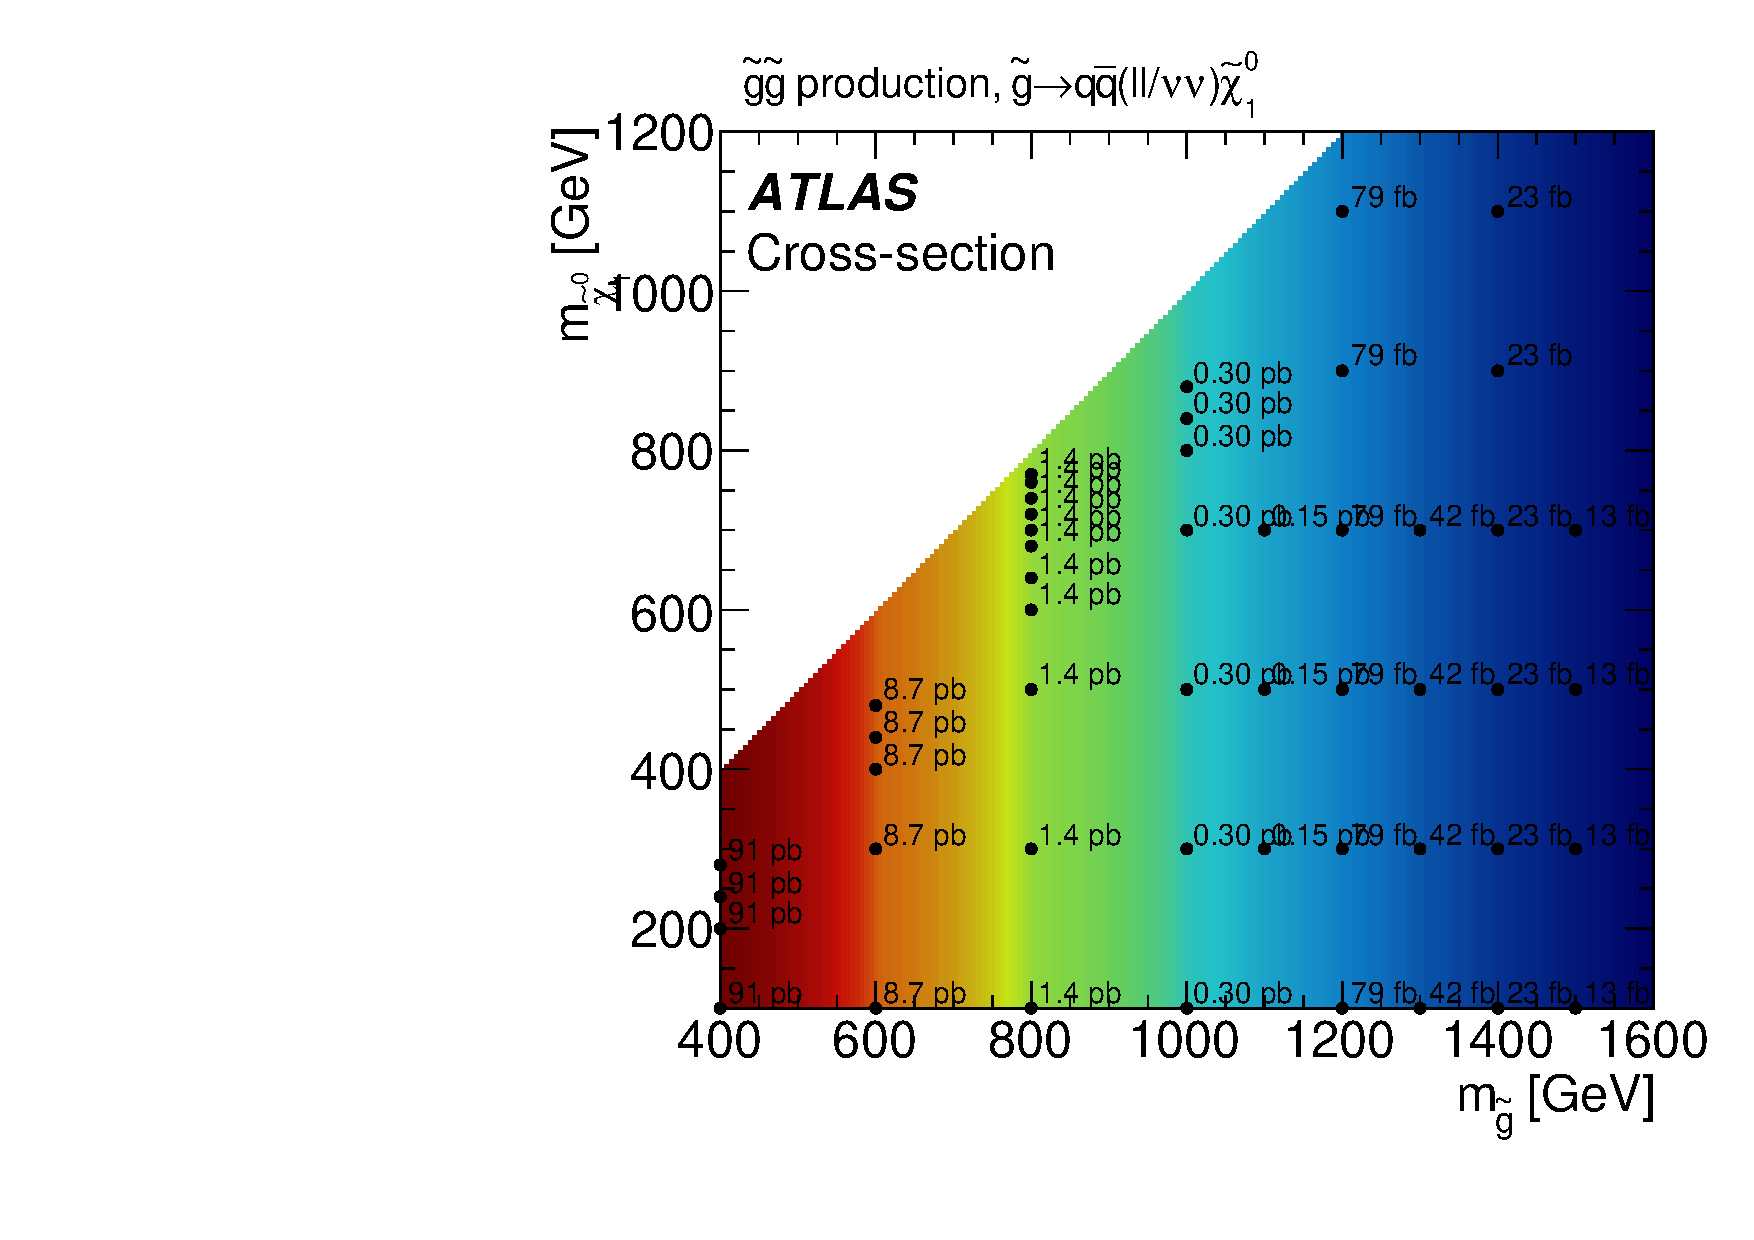
\includegraphics[width=0.37\textwidth]{PUB/FIGURES/HEPDATA/xsection_SR0b3j.pdf}}
\subfigure{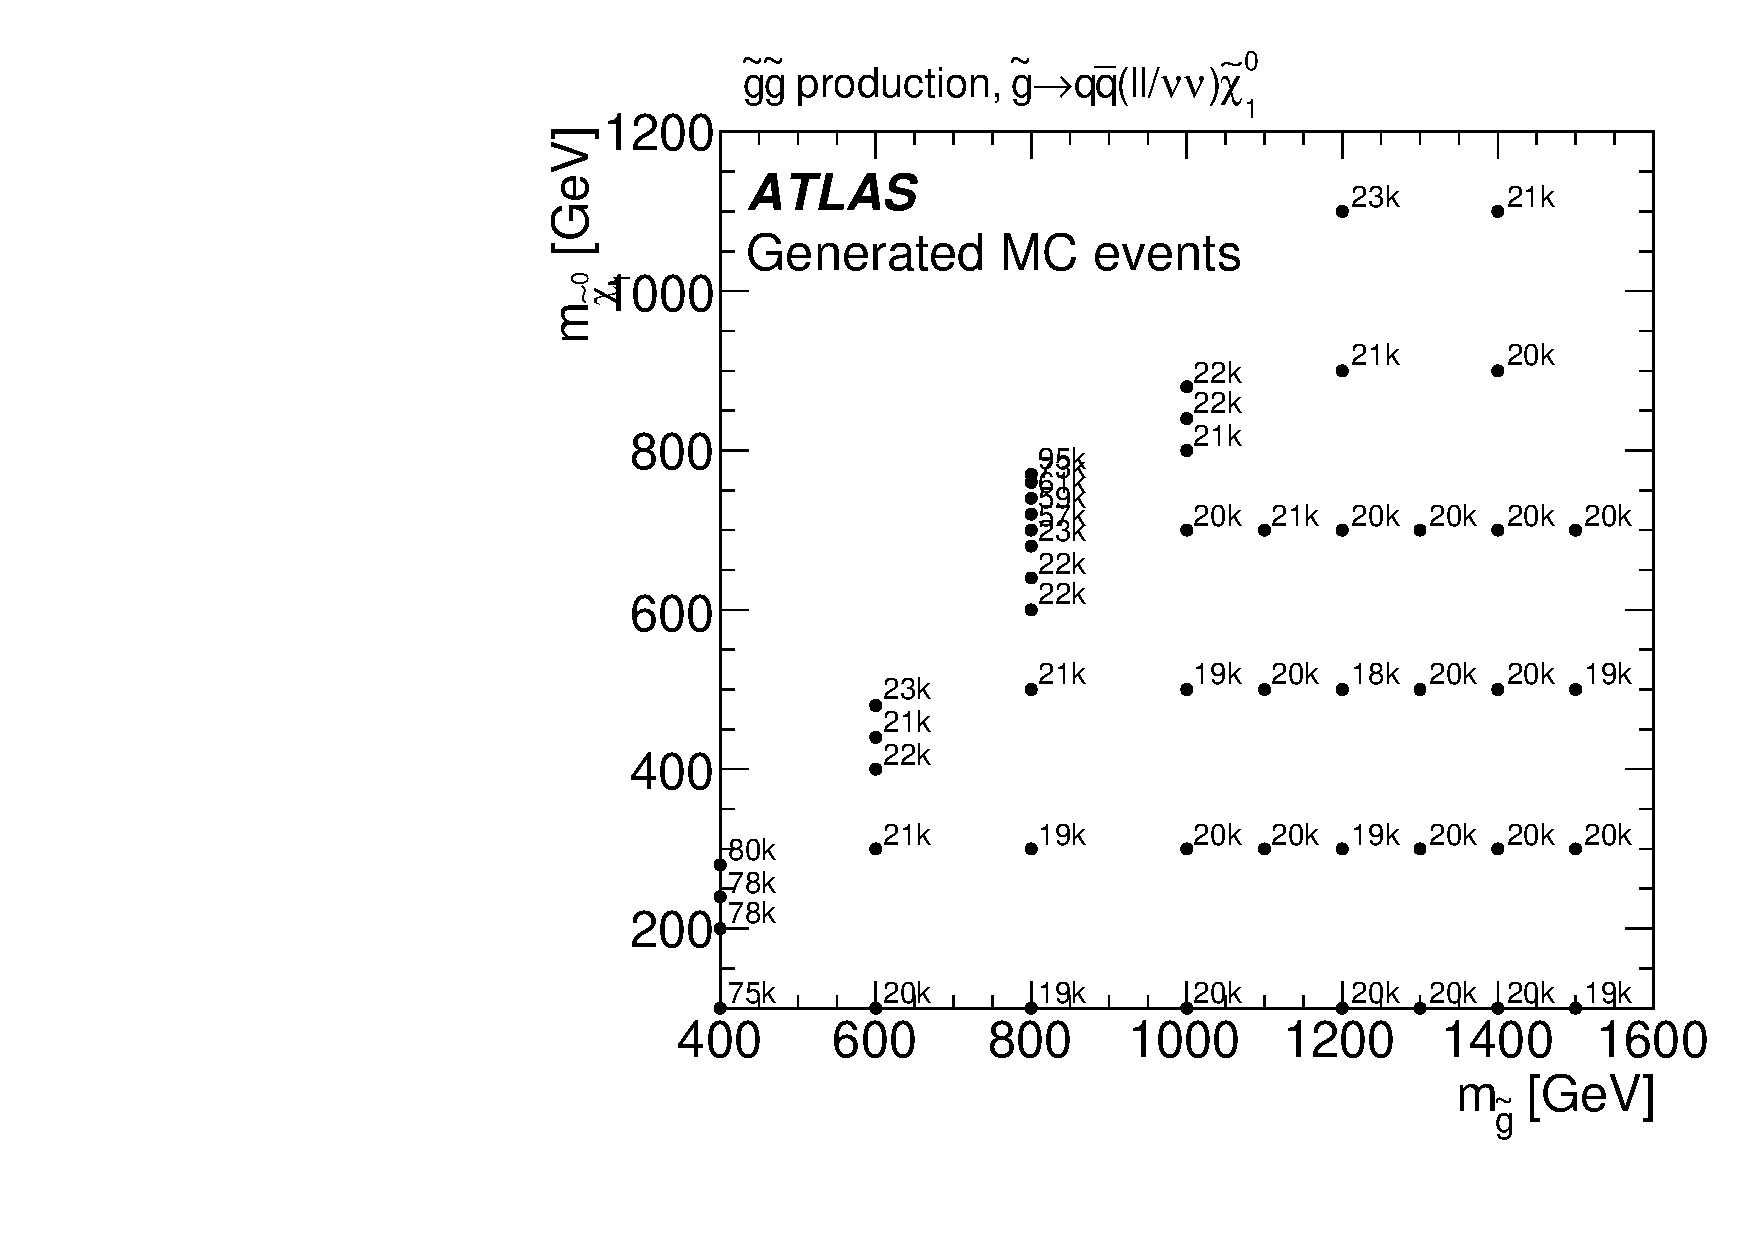
\includegraphics[width=0.37\textwidth]{PUB/FIGURES/HEPDATA/mcstats_SR0b3j.pdf}}
\subfigure{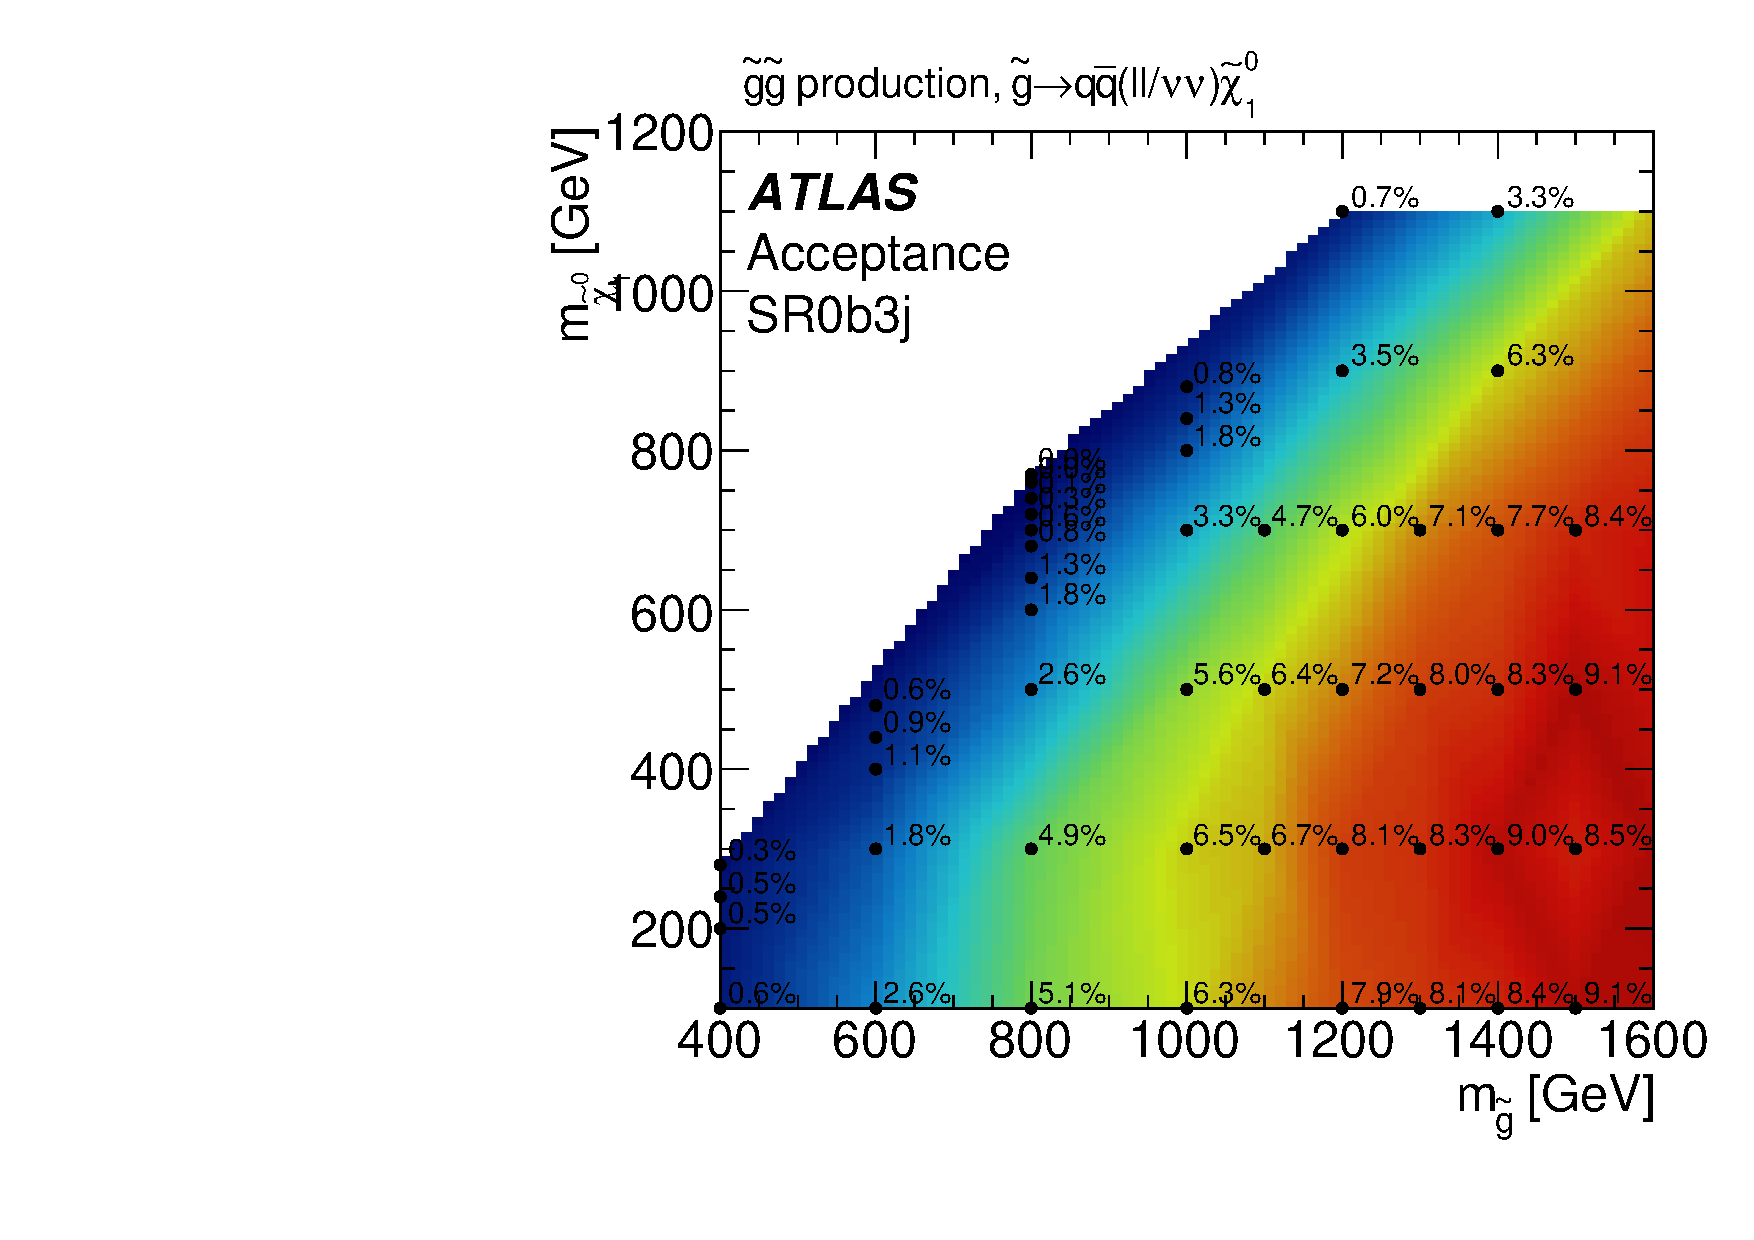
\includegraphics[width=0.37\textwidth]{PUB/FIGURES/HEPDATA/acceptance_SR0b3j.pdf}}
\subfigure{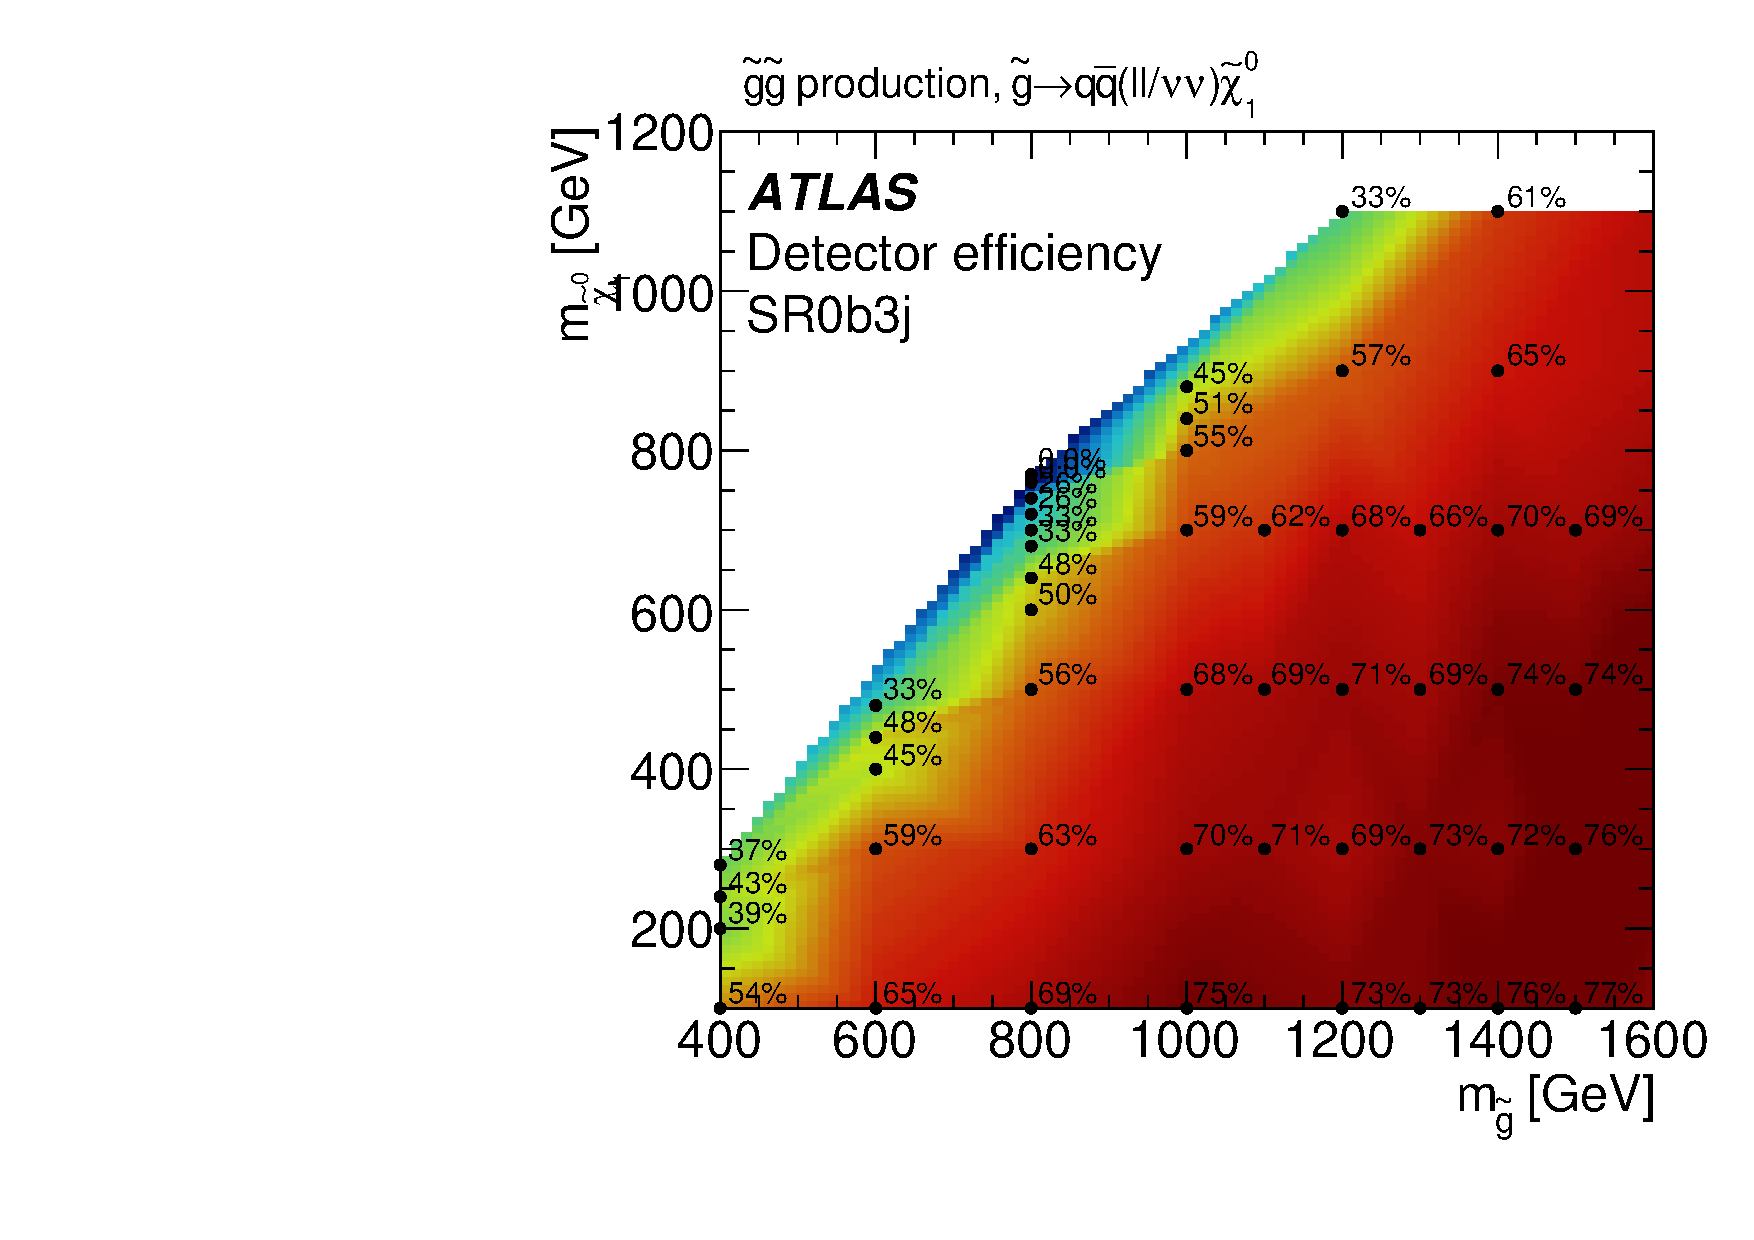
\includegraphics[width=0.37\textwidth]{PUB/FIGURES/HEPDATA/efficiency_SR0b3j.pdf}}
\subfigure{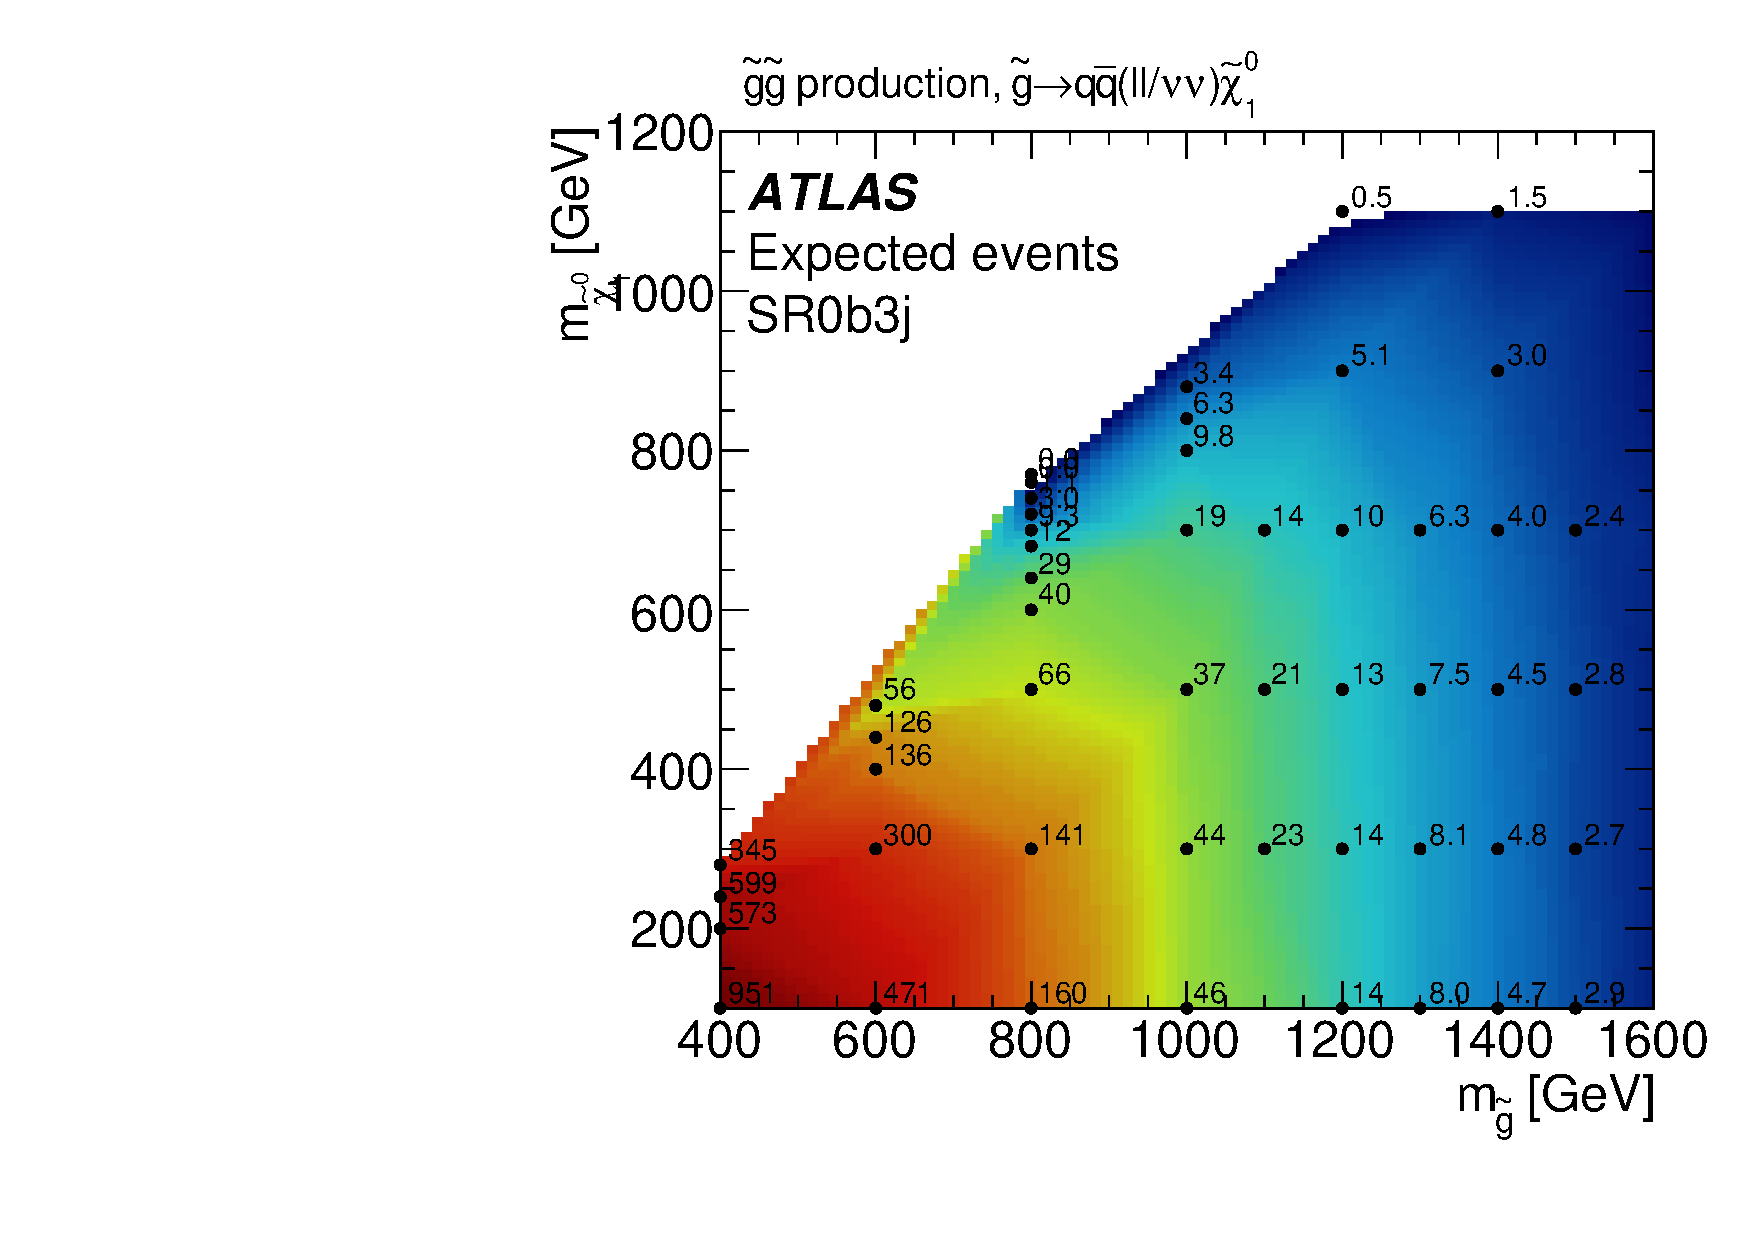
\includegraphics[width=0.37\textwidth]{PUB/FIGURES/HEPDATA/yield_SR0b3j.pdf}}
\subfigure{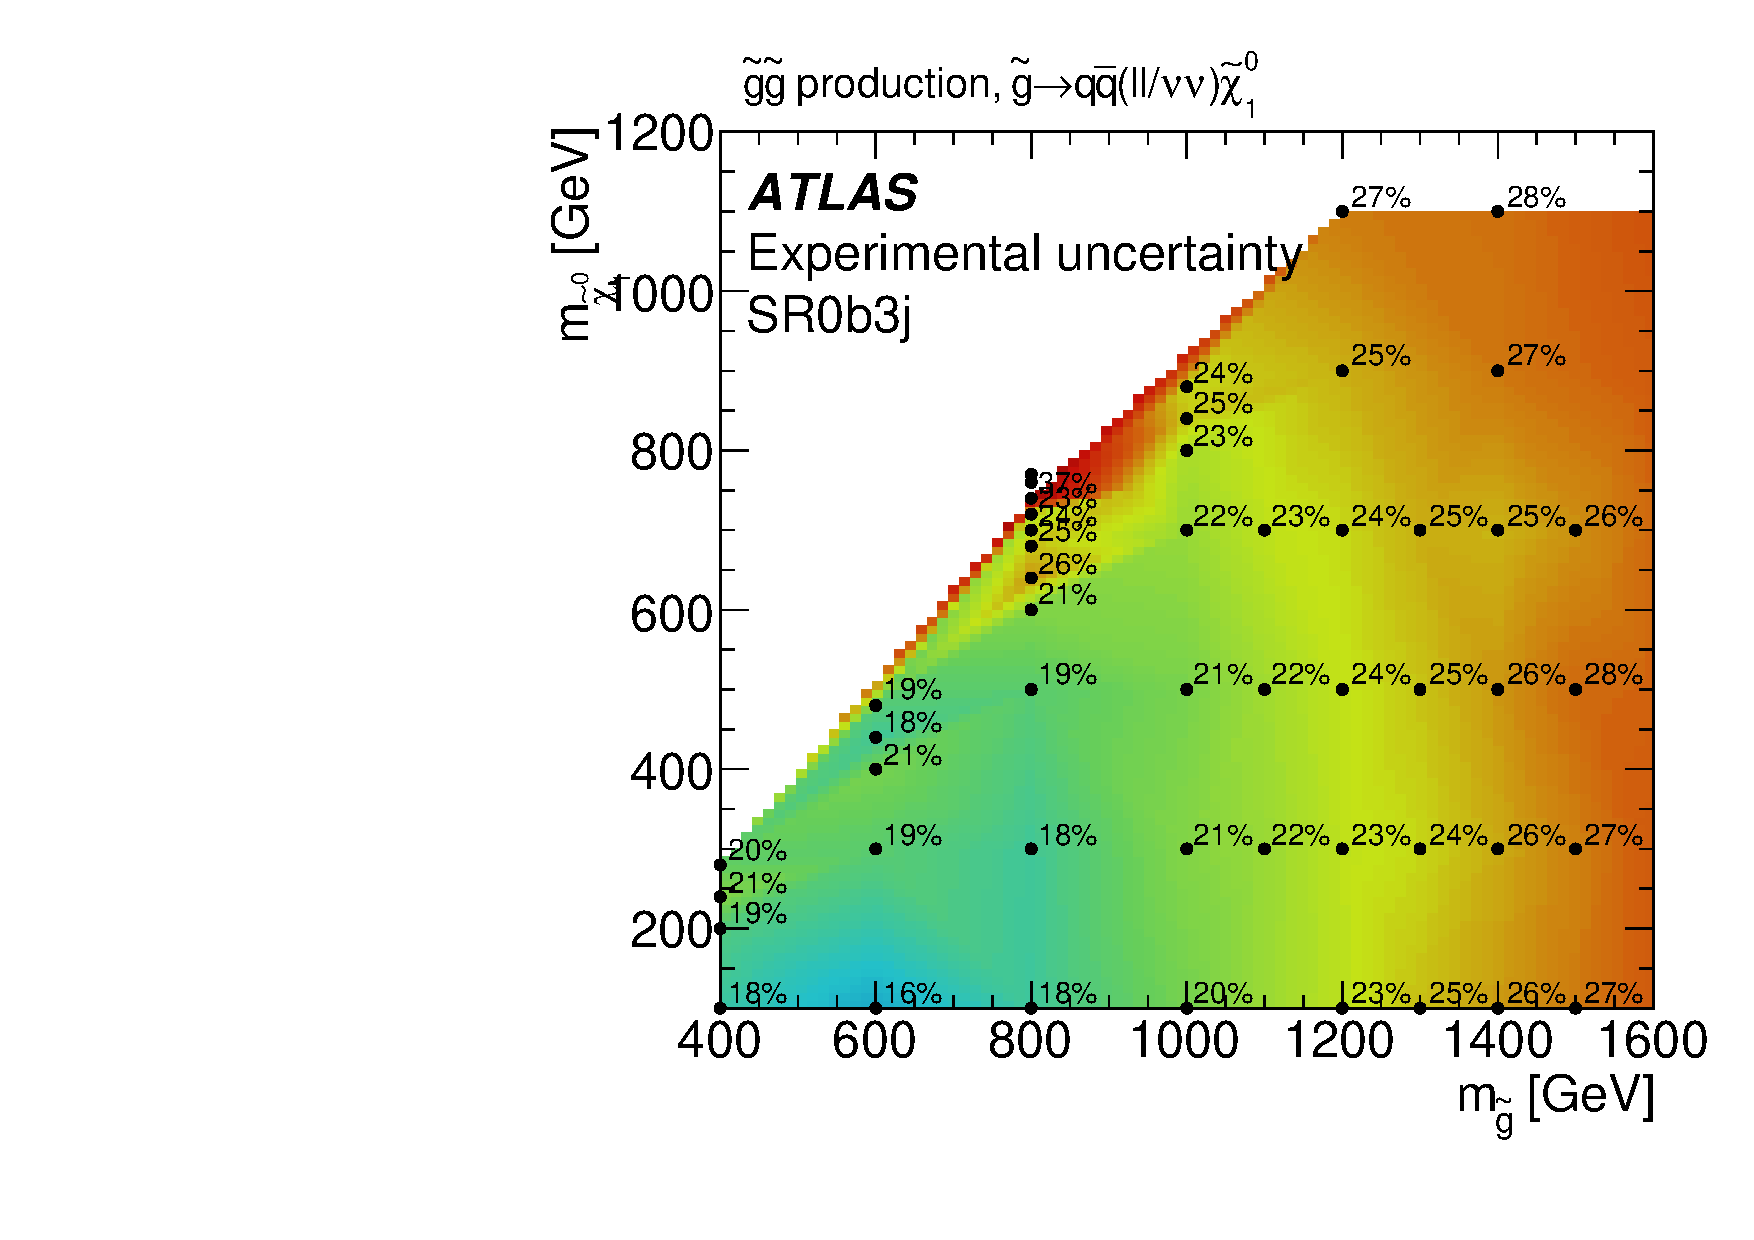
\includegraphics[width=0.37\textwidth]{PUB/FIGURES/HEPDATA/mcsyst_SR0b3j.pdf}}
\caption{SUSY scenario with $\gluino\gluino$ production and $\gluino\to q\bar q\ell\ell\ninoone$ decay: 
production cross-section (top left), number of generated MC events (top right), 
signal acceptance (middle left) and reconstruction efficiency (middle right) in the signal region SR0b3j, 
corresponding expected signal yield (bottom left) and associated uncertainty due to experimental sources (bottom right). 
The benchmark scenarios used to set exclusion limits are materialized by black dot markers. 
Acceptance and efficiency are defined as in appendix~A of~\cite{SUSY-2013-19}.}
\label{HEPData_SR0b3j}
\end{figure}

% SR0b5j PUB/FIGURES/HEPData plots
\begin{figure}[p]
\centering
\subfigure{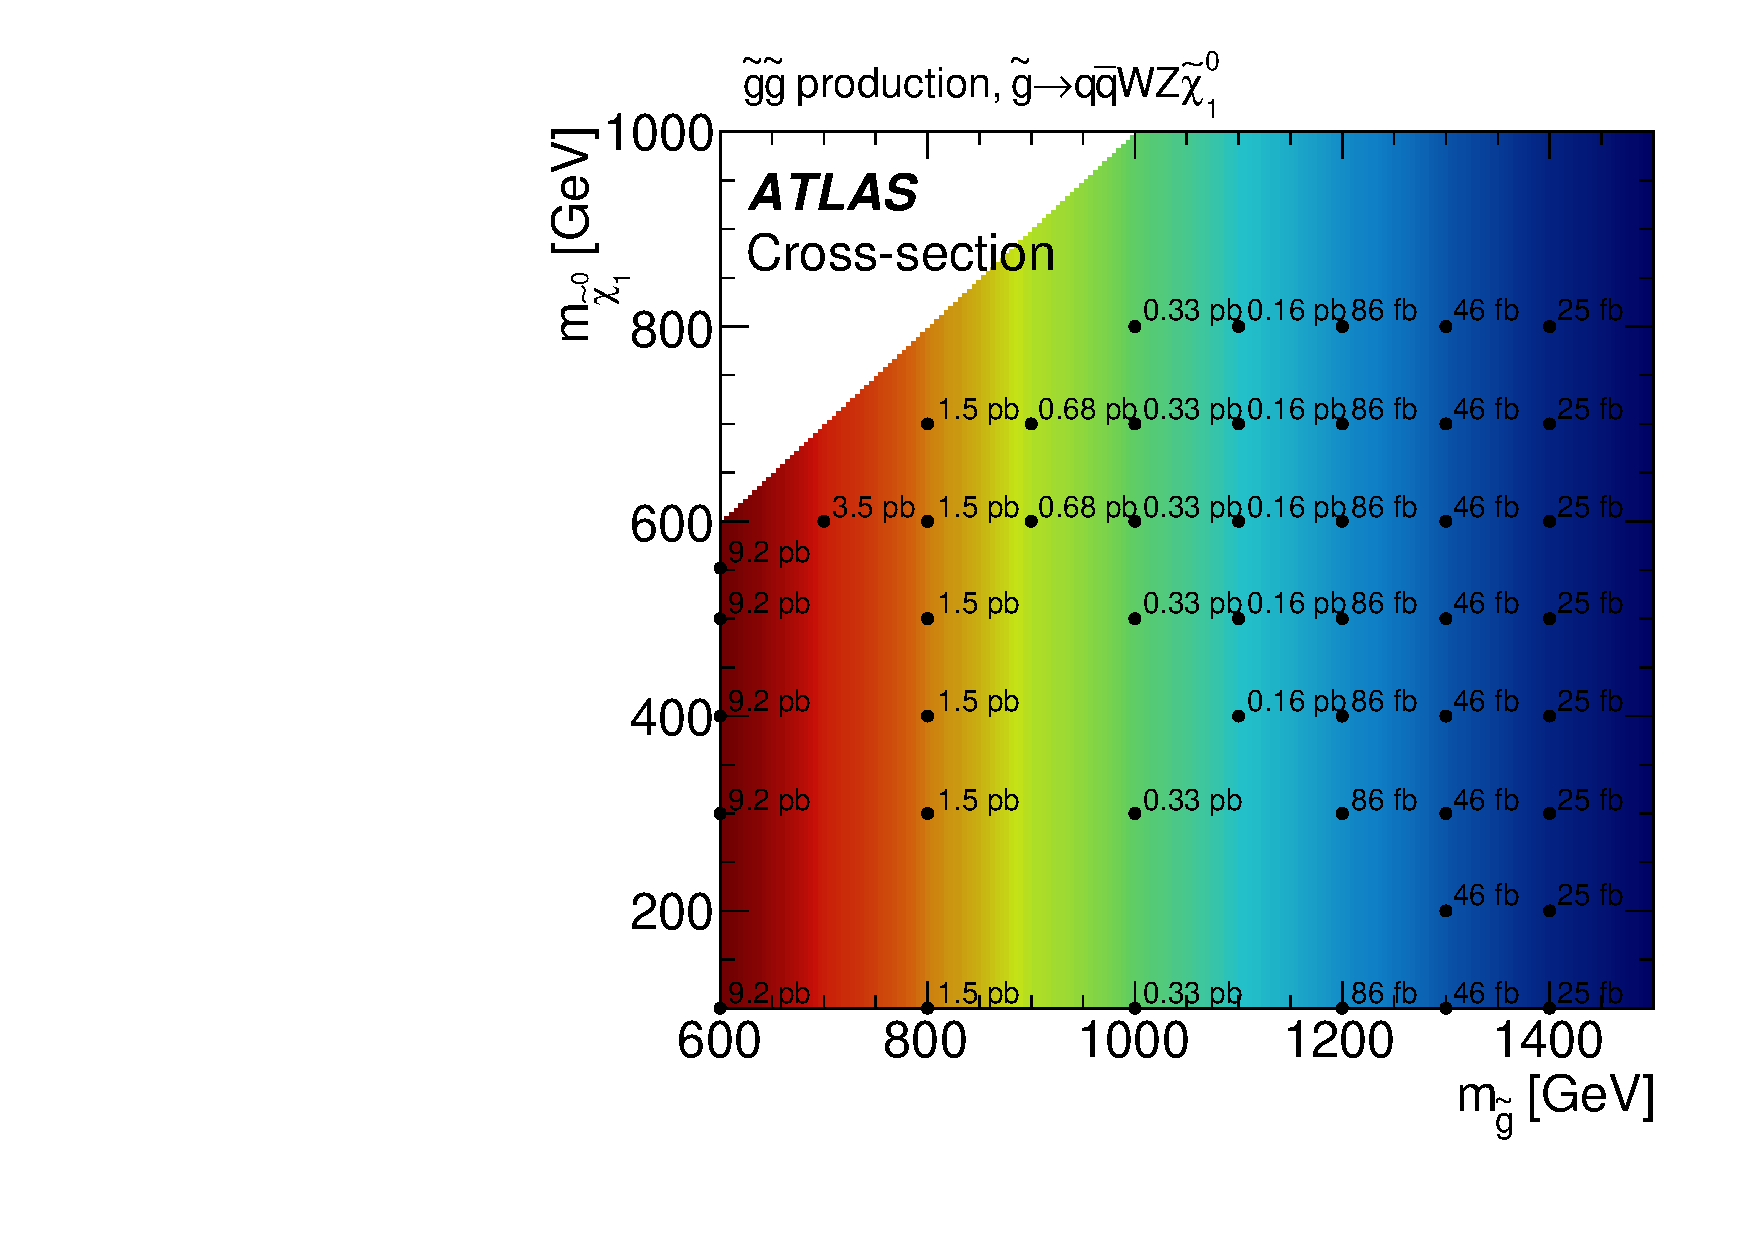
\includegraphics[width=0.37\textwidth]{PUB/FIGURES/HEPDATA/xsection_SR0b5j.pdf}}
\subfigure{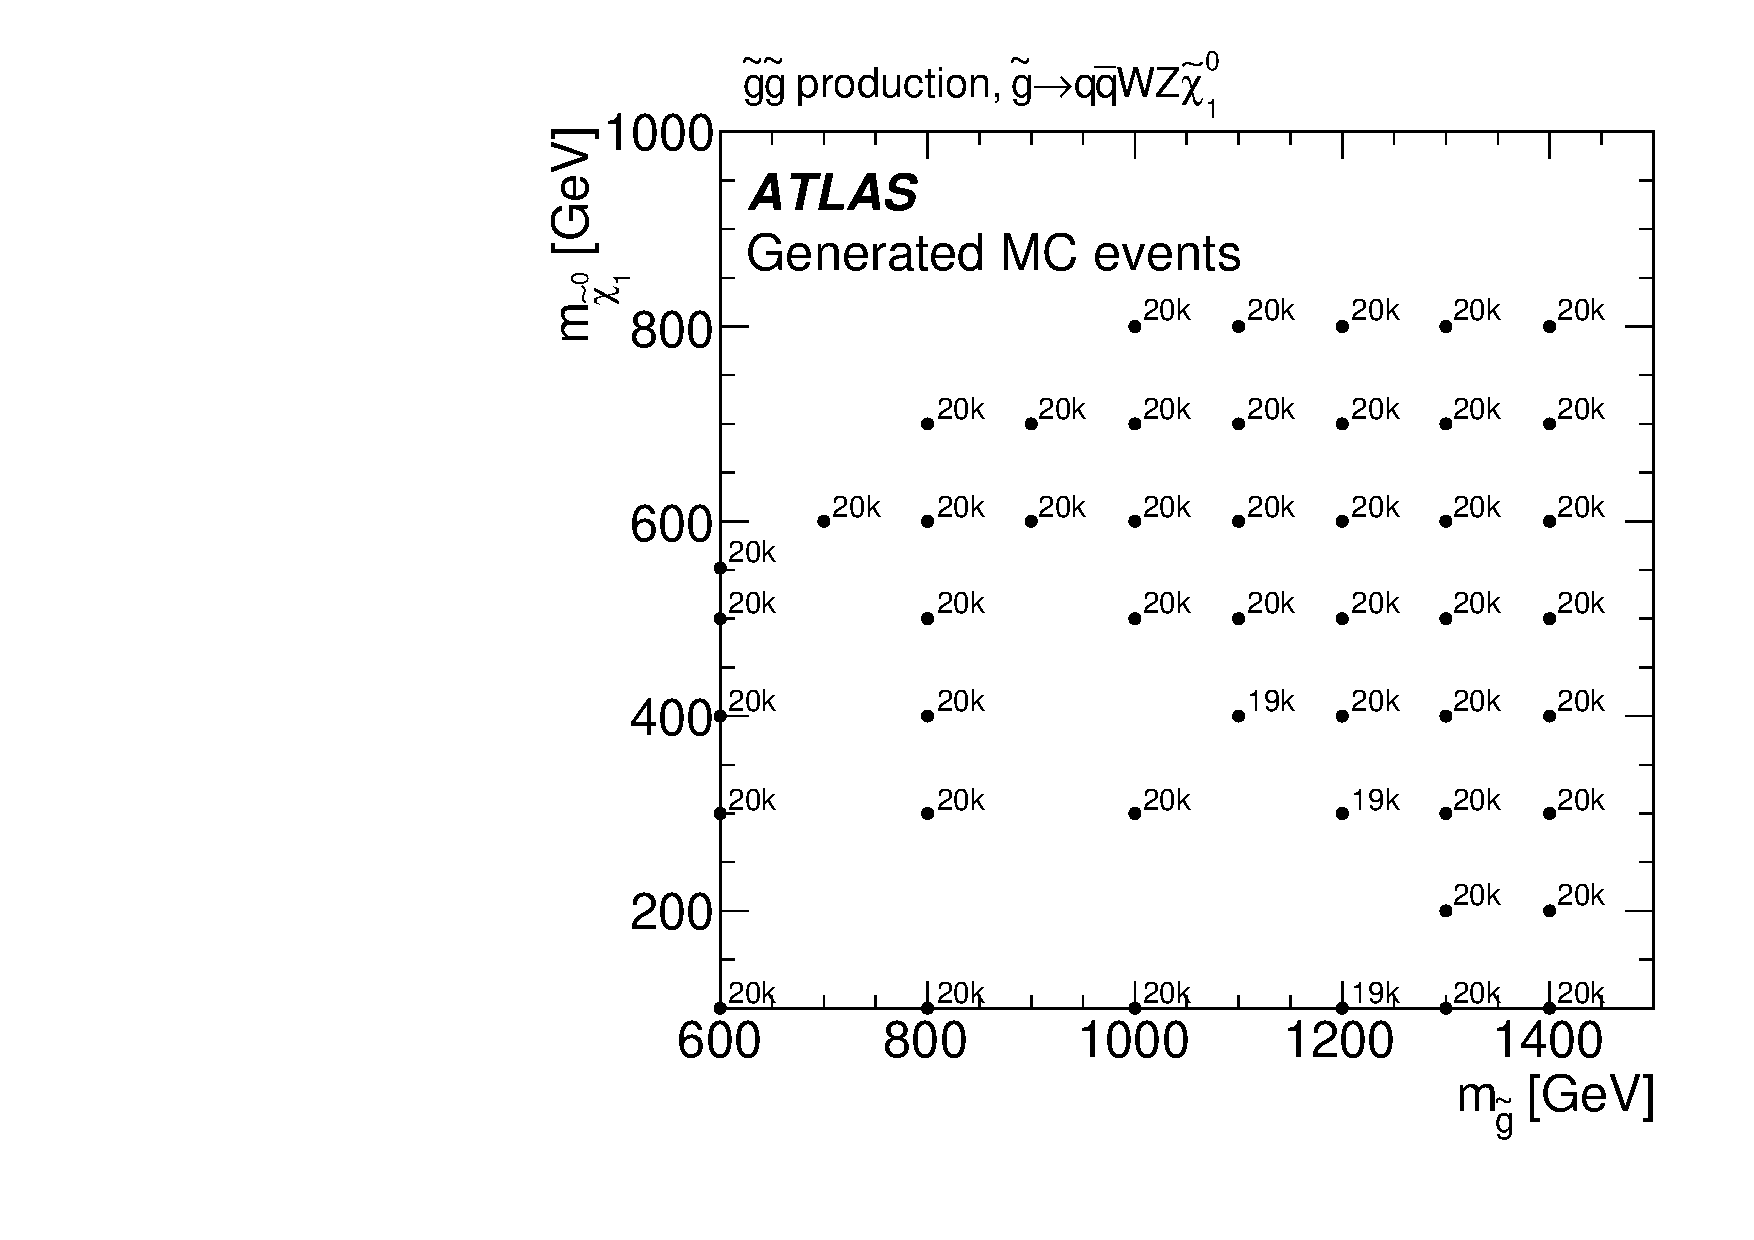
\includegraphics[width=0.37\textwidth]{PUB/FIGURES/HEPDATA/mcstats_SR0b5j.pdf}}
\subfigure{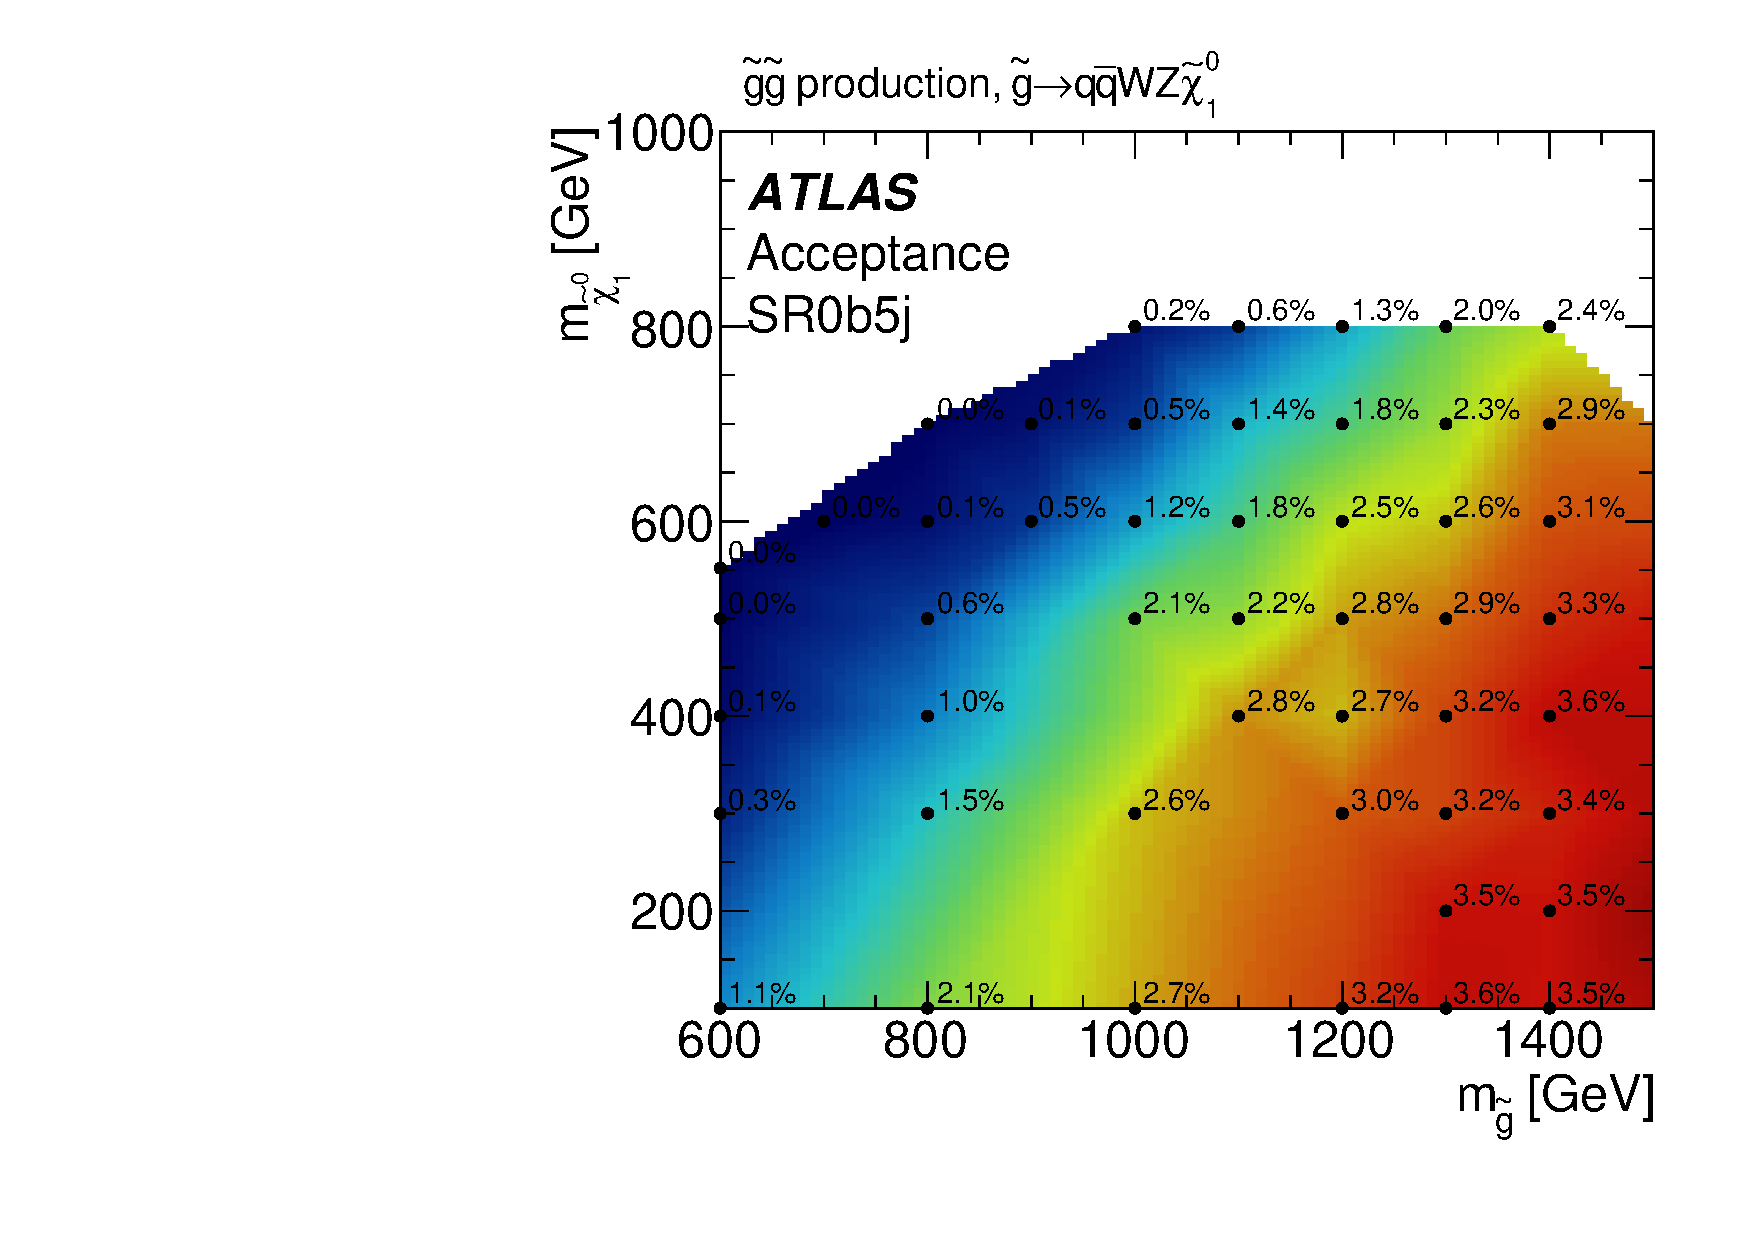
\includegraphics[width=0.37\textwidth]{PUB/FIGURES/HEPDATA/acceptance_SR0b5j.pdf}}
\subfigure{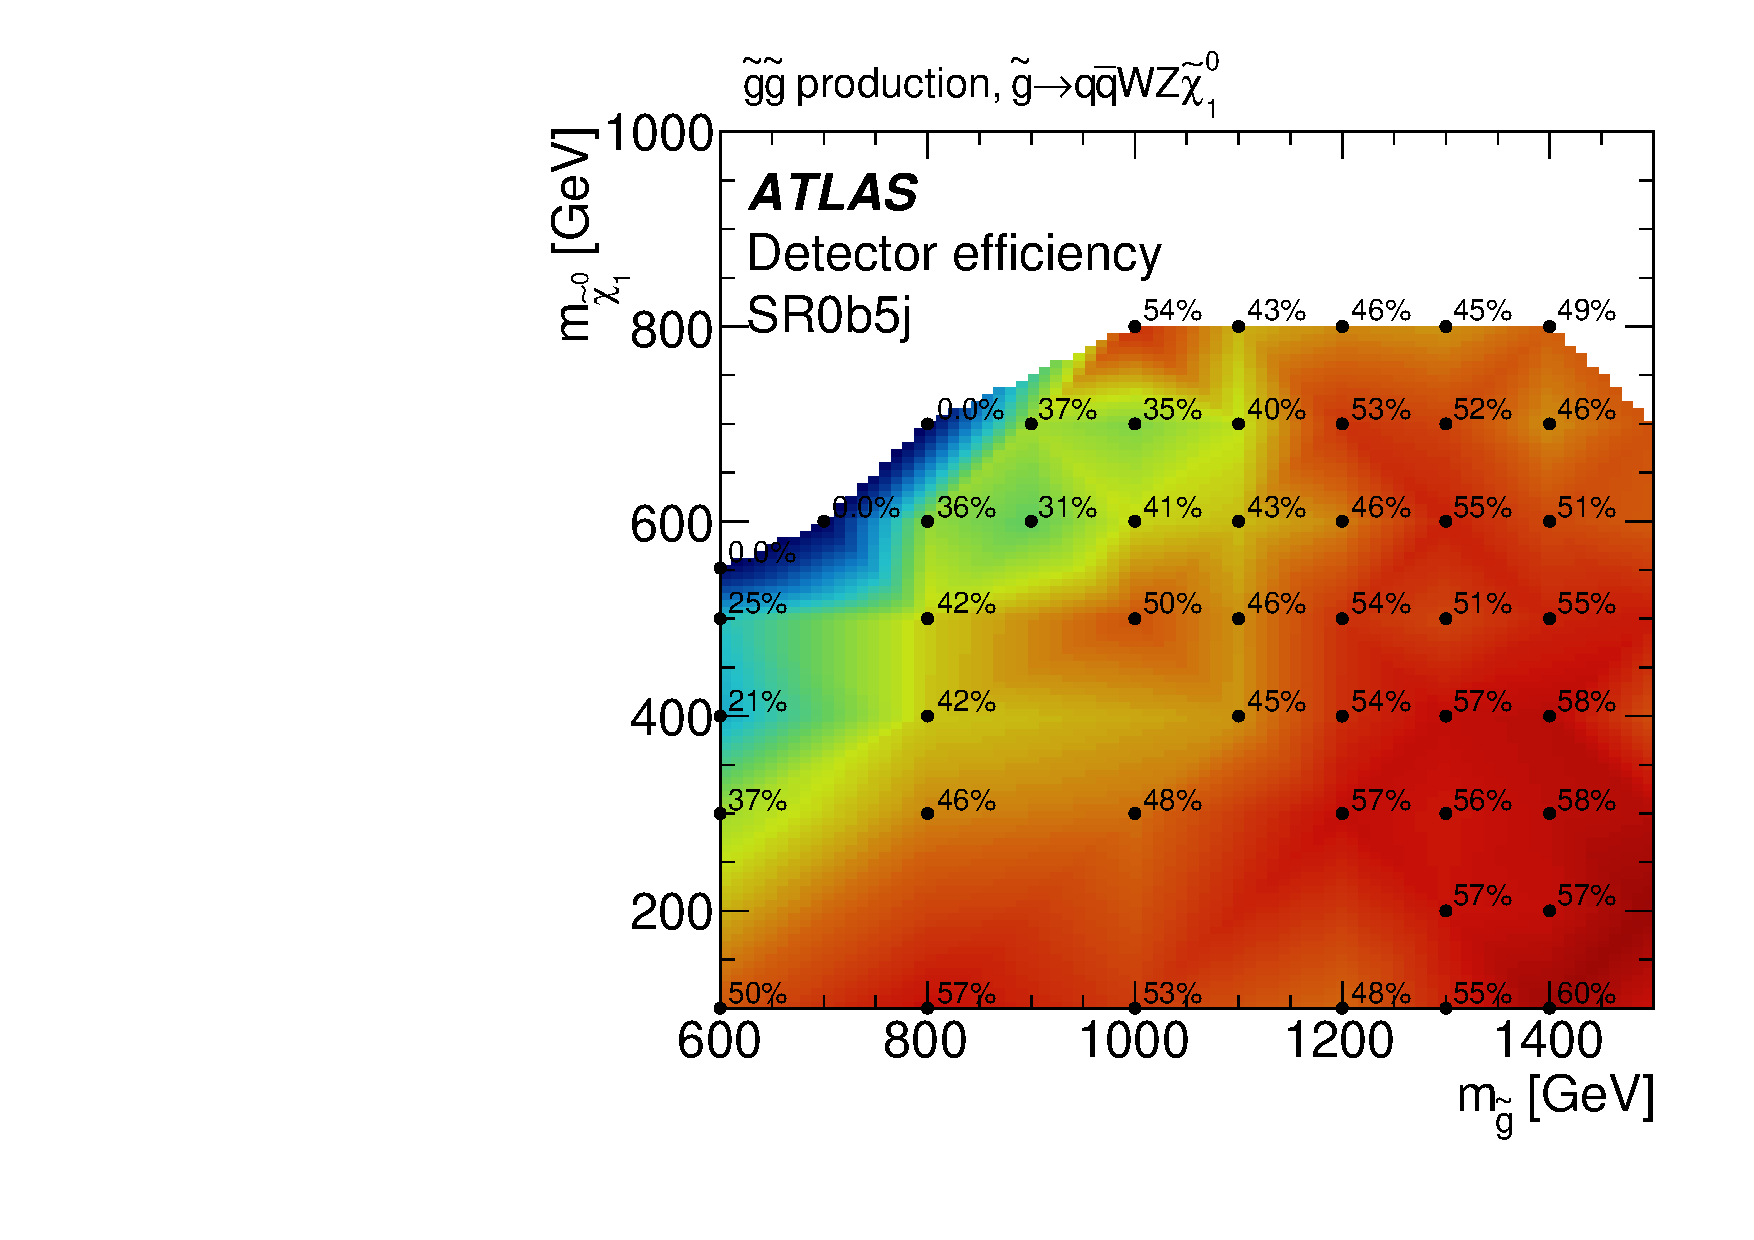
\includegraphics[width=0.37\textwidth]{PUB/FIGURES/HEPDATA/efficiency_SR0b5j.pdf}}
\subfigure{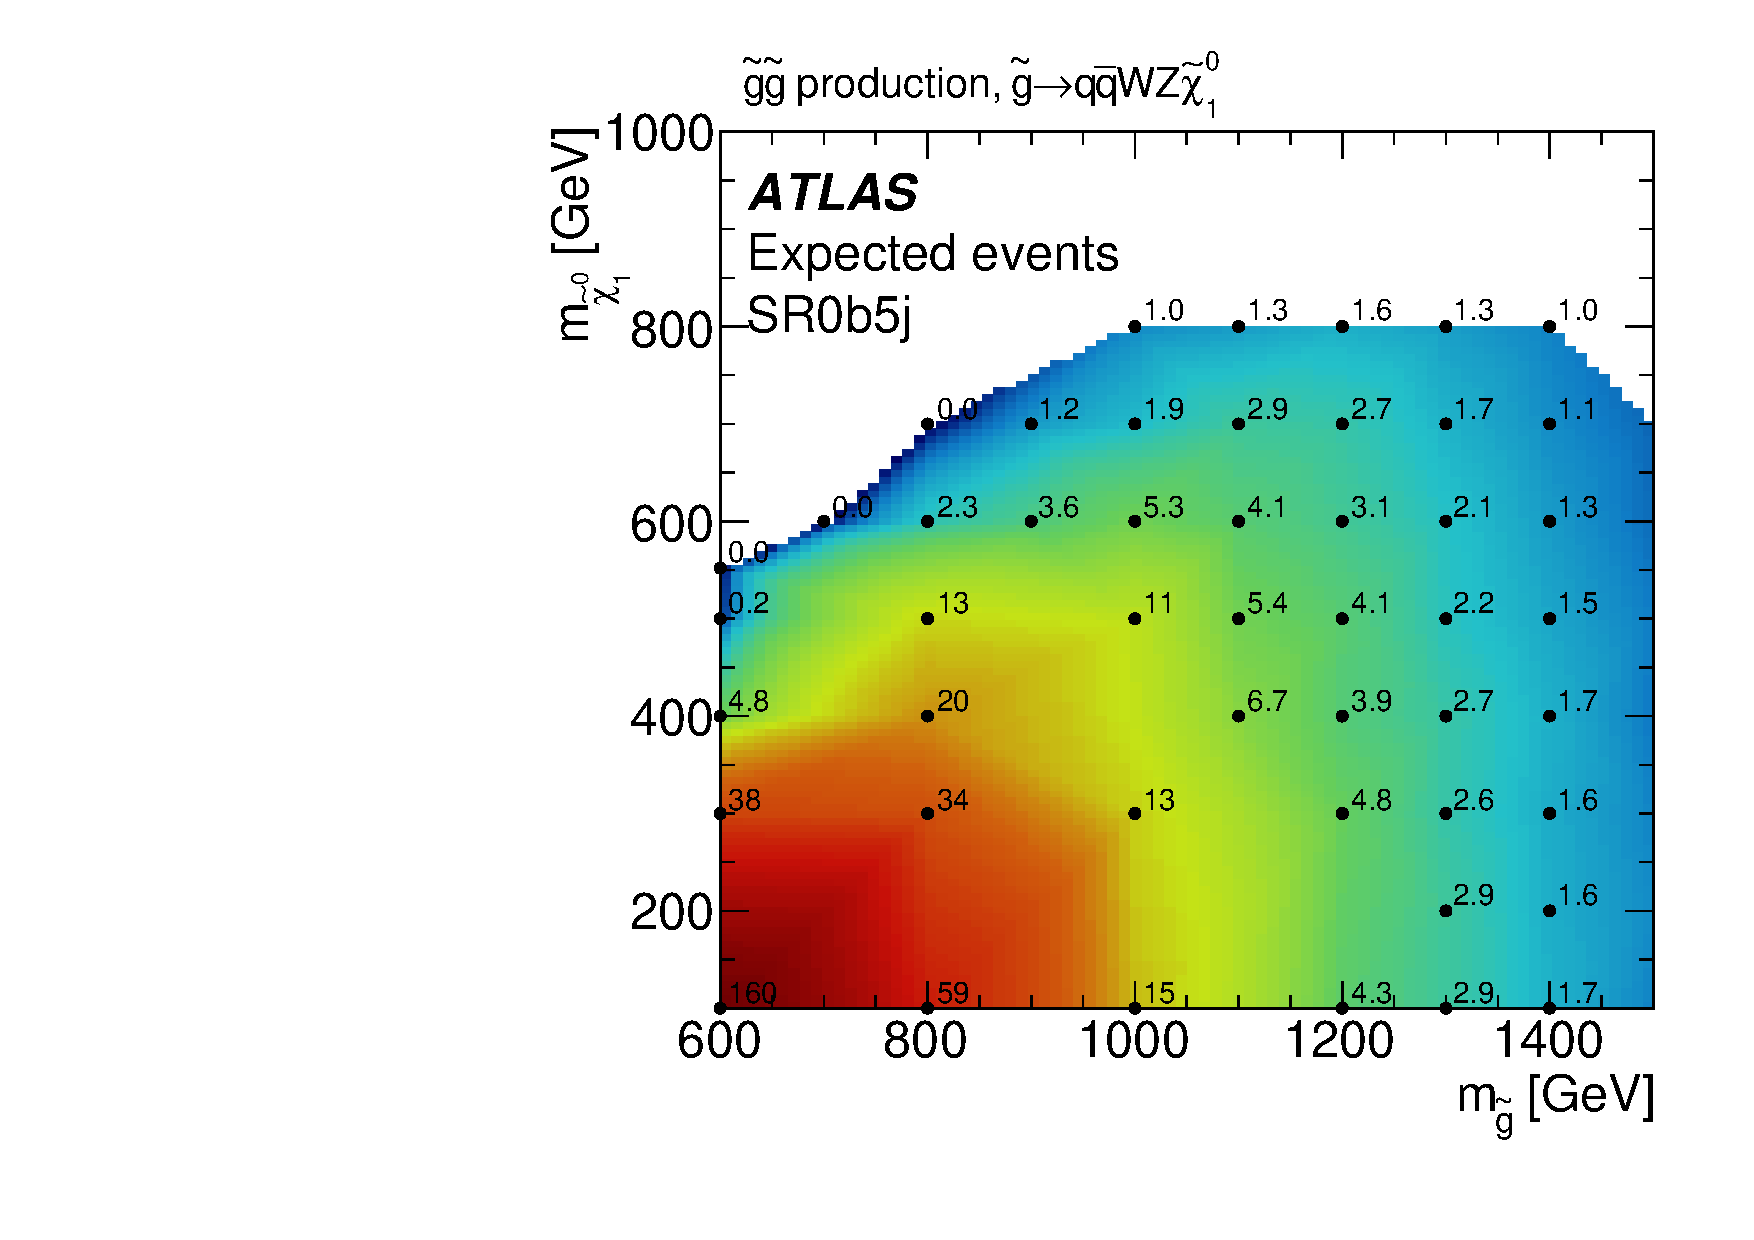
\includegraphics[width=0.37\textwidth]{PUB/FIGURES/HEPDATA/yield_SR0b5j.pdf}}
\subfigure{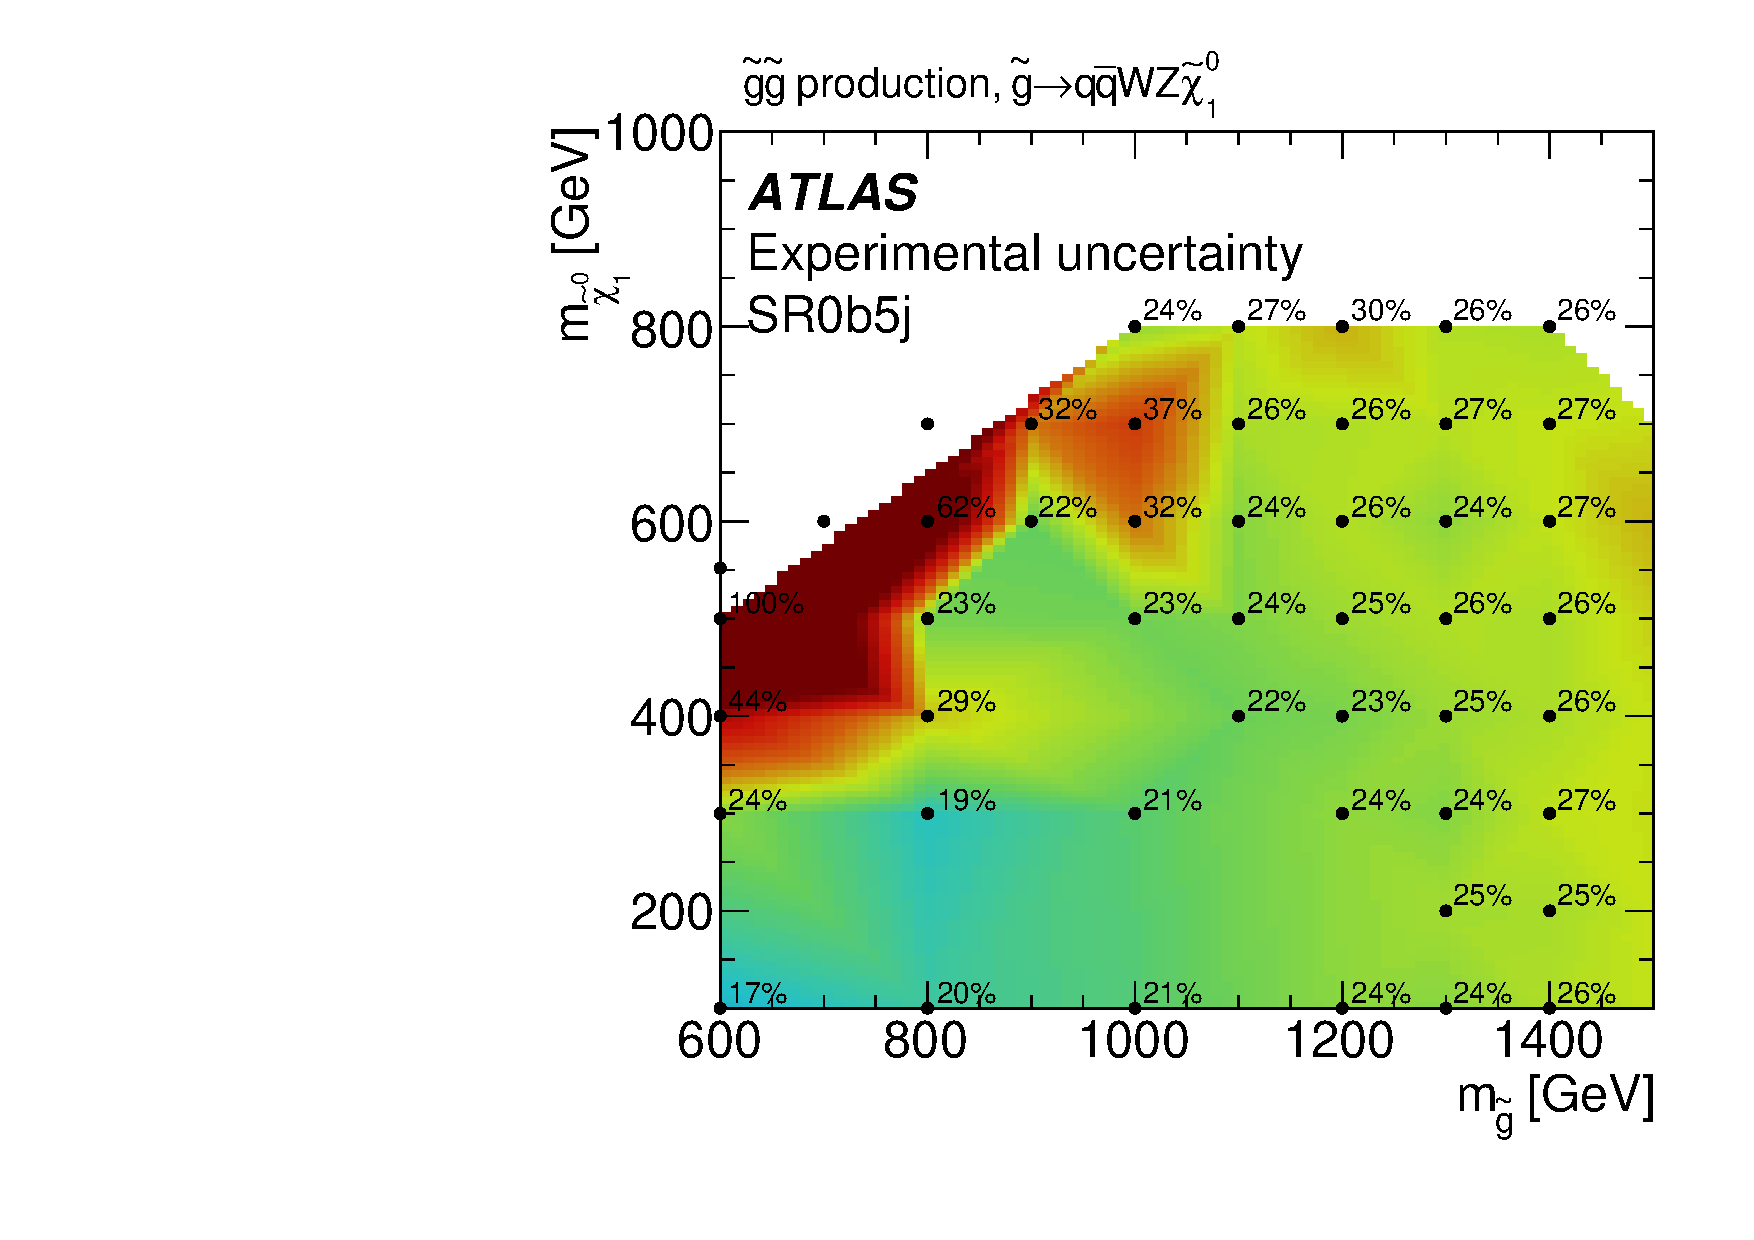
\includegraphics[width=0.37\textwidth]{PUB/FIGURES/HEPDATA/mcsyst_SR0b5j.pdf}}
\caption{SUSY scenario with $\gluino\gluino$ production and $\gluino\to q\bar qWZ\ninoone$ decay: 
production cross-section (top left), number of generated MC events (top right), 
signal acceptance (middle left) and reconstruction efficiency (middle right) in the signal region SR0b5j, 
corresponding expected signal yield (bottom left) and associated uncertainty due to experimental sources (bottom right). 
The benchmark scenarios used to set exclusion limits are materialized by black dot markers. 
Acceptance and efficiency are defined as in appendix~A of~\cite{SUSY-2013-19}.}
\label{HEPData_SR0b5j} 
\end{figure}

% SR1b PUB/FIGURES/HEPData plots
\begin{figure}[p]
\centering
\subfigure{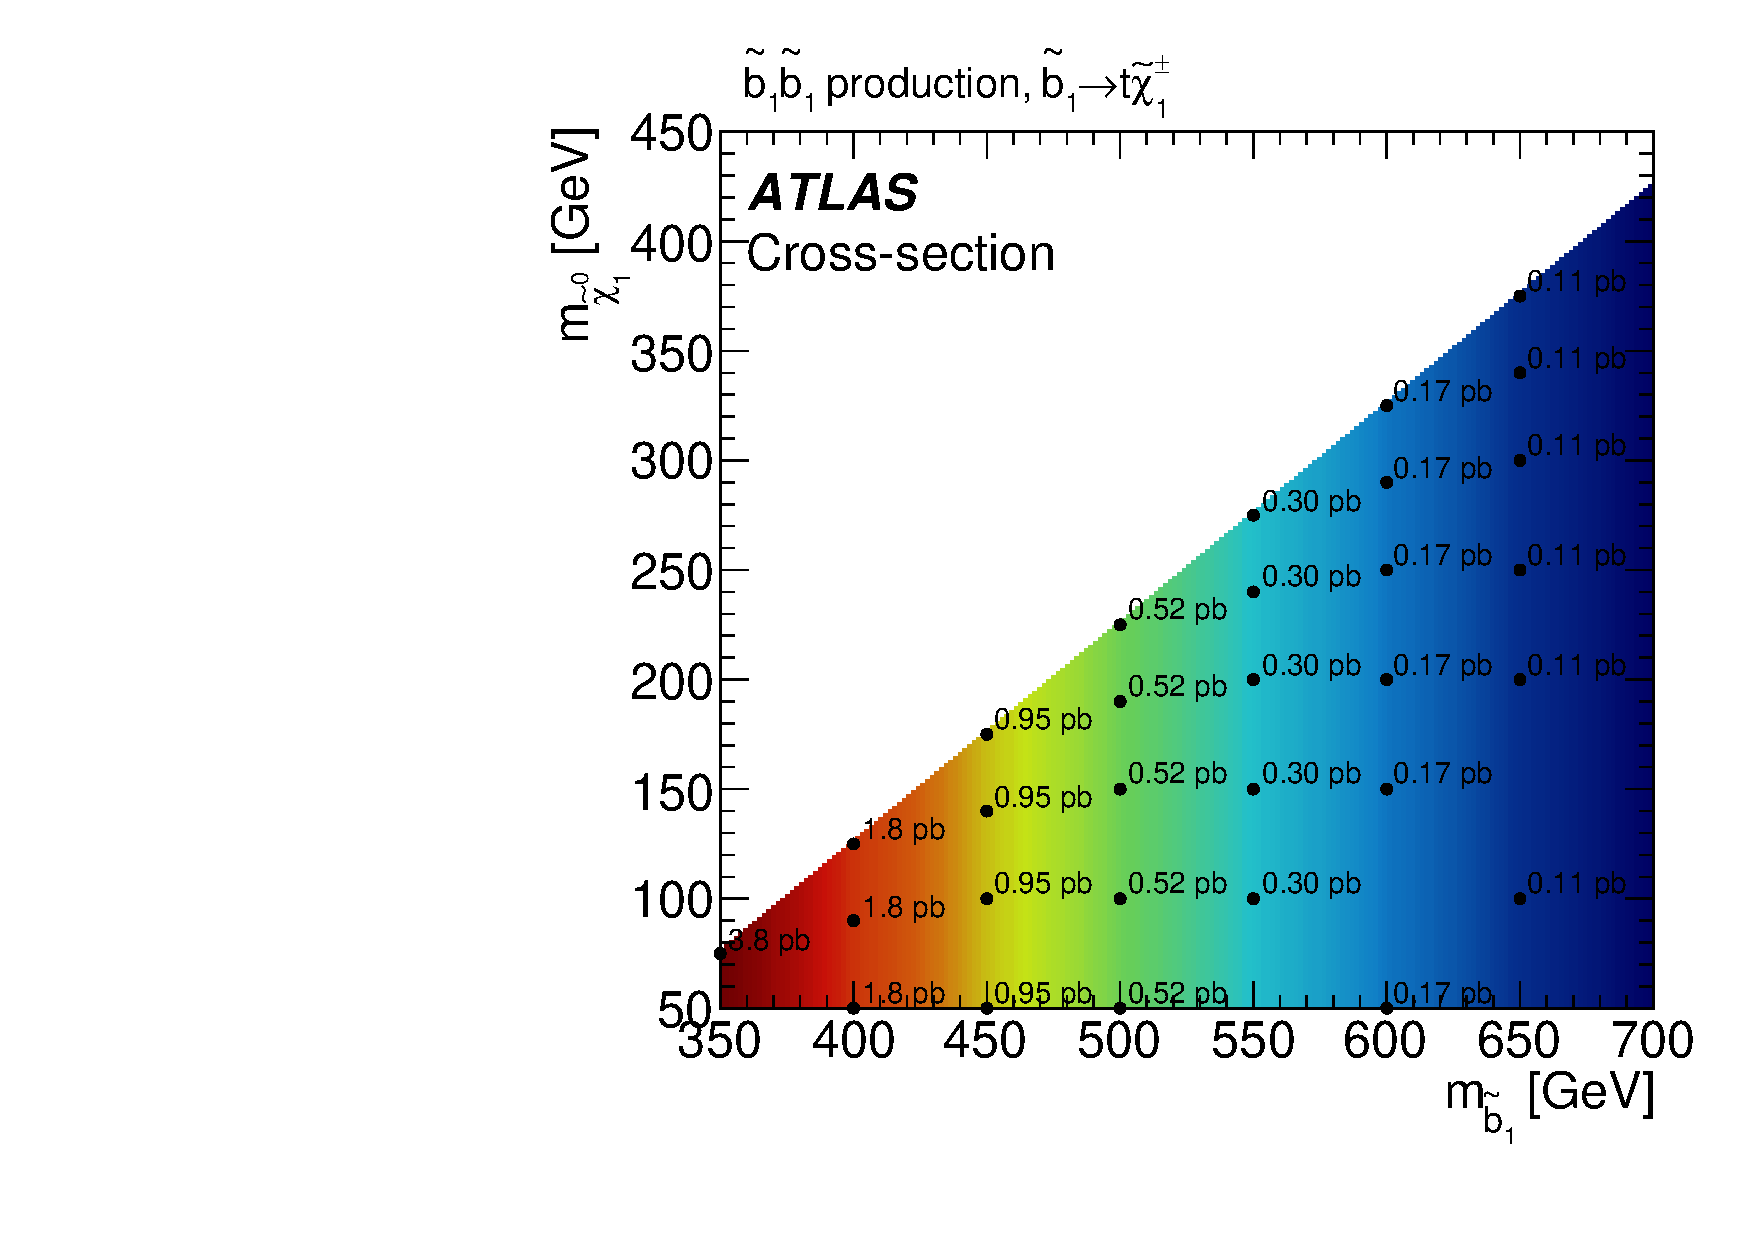
\includegraphics[width=0.37\textwidth]{PUB/FIGURES/HEPDATA/xsection_SR1b.pdf}}
\subfigure{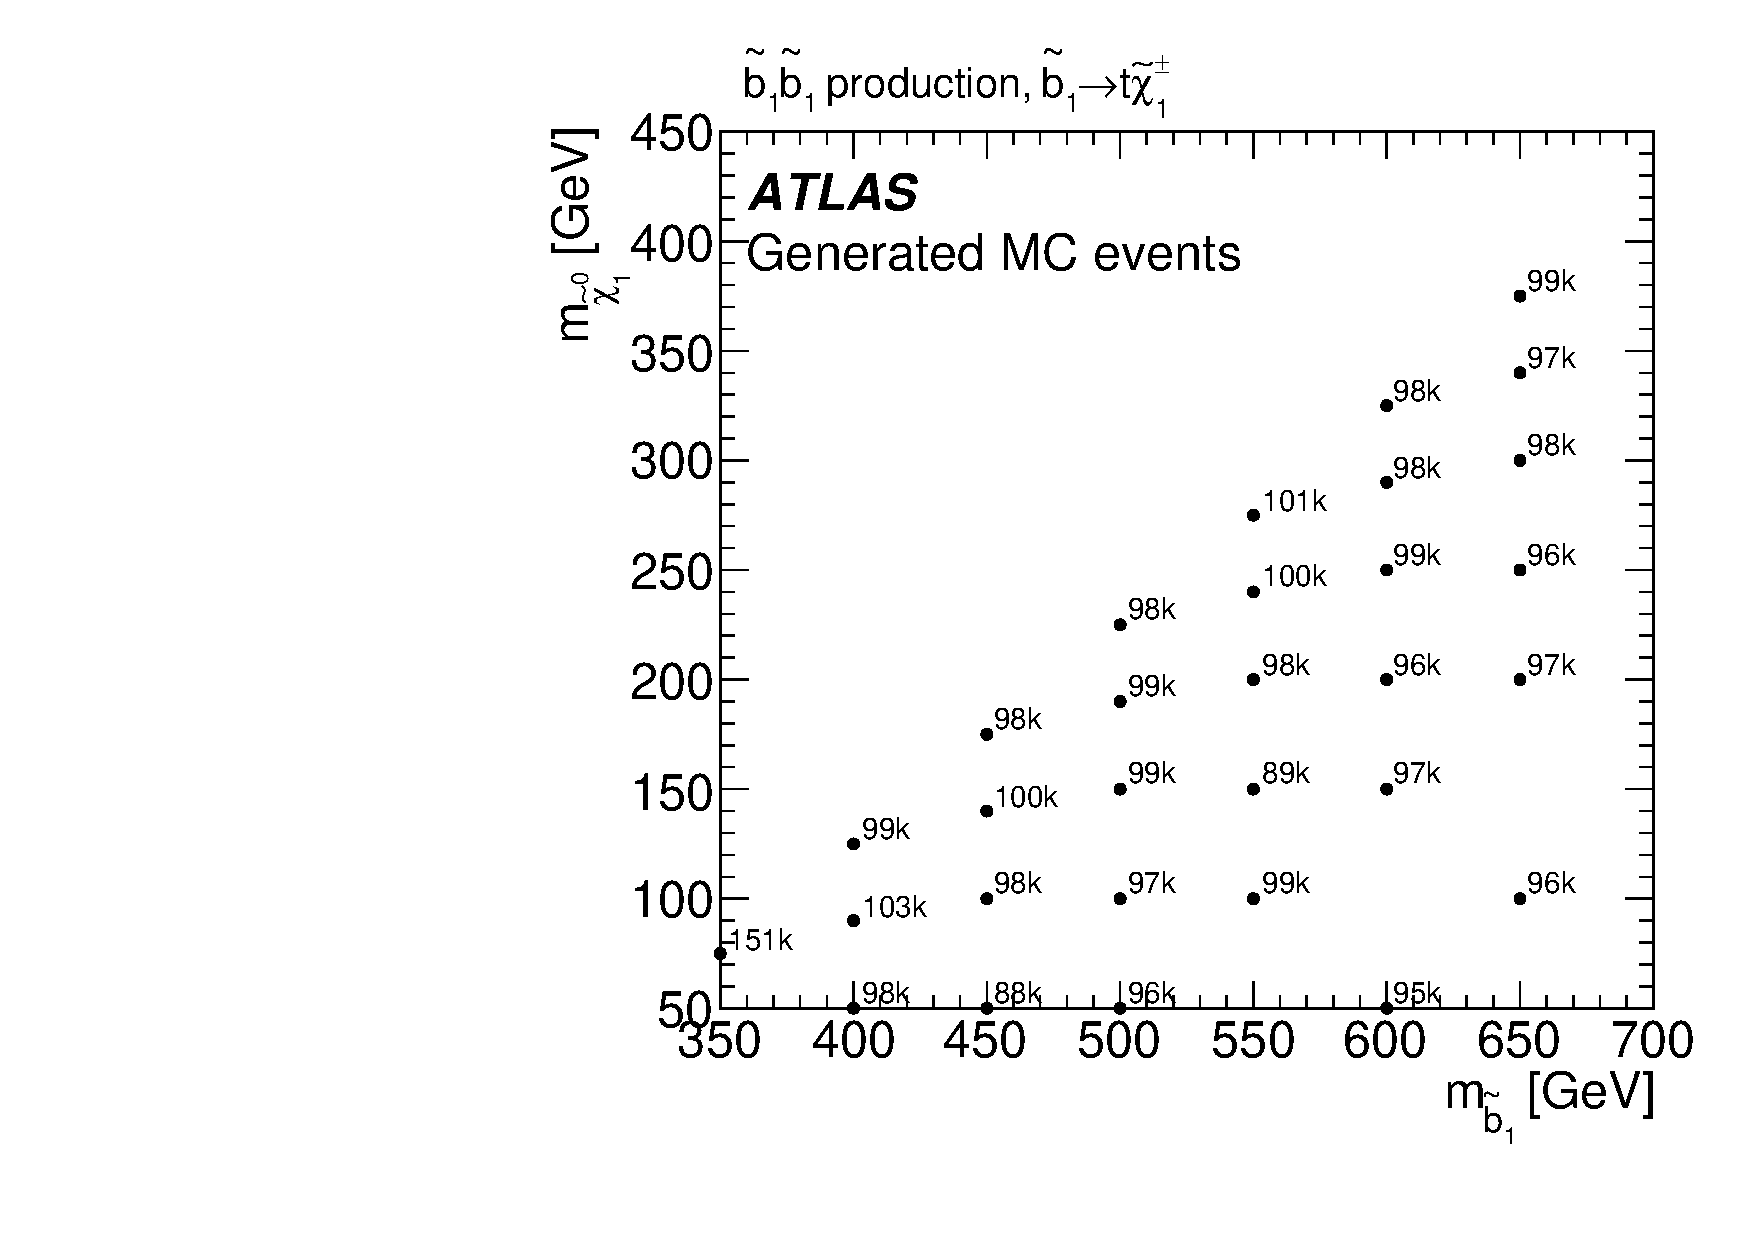
\includegraphics[width=0.37\textwidth]{PUB/FIGURES/HEPDATA/mcstats_SR1b.pdf}}
\subfigure{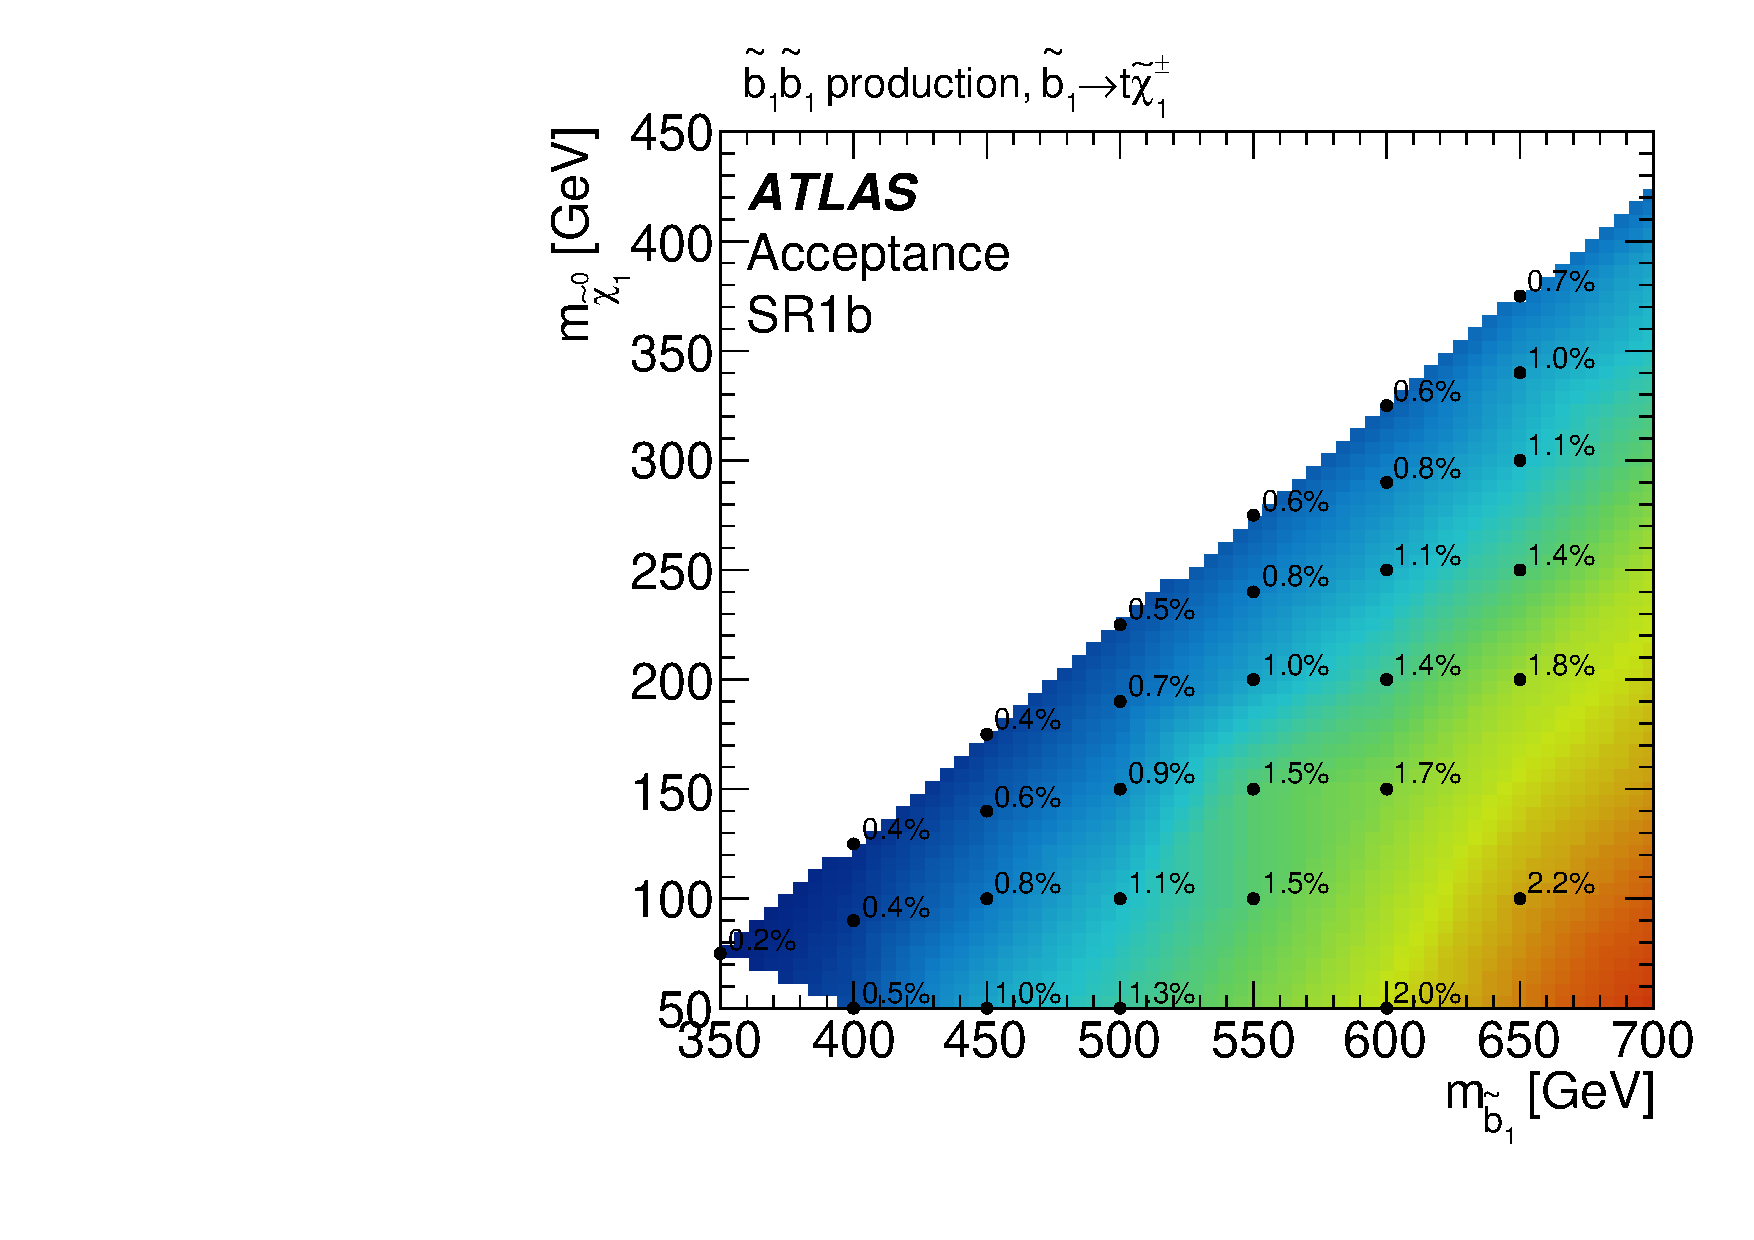
\includegraphics[width=0.37\textwidth]{PUB/FIGURES/HEPDATA/acceptance_SR1b.pdf}}
\subfigure{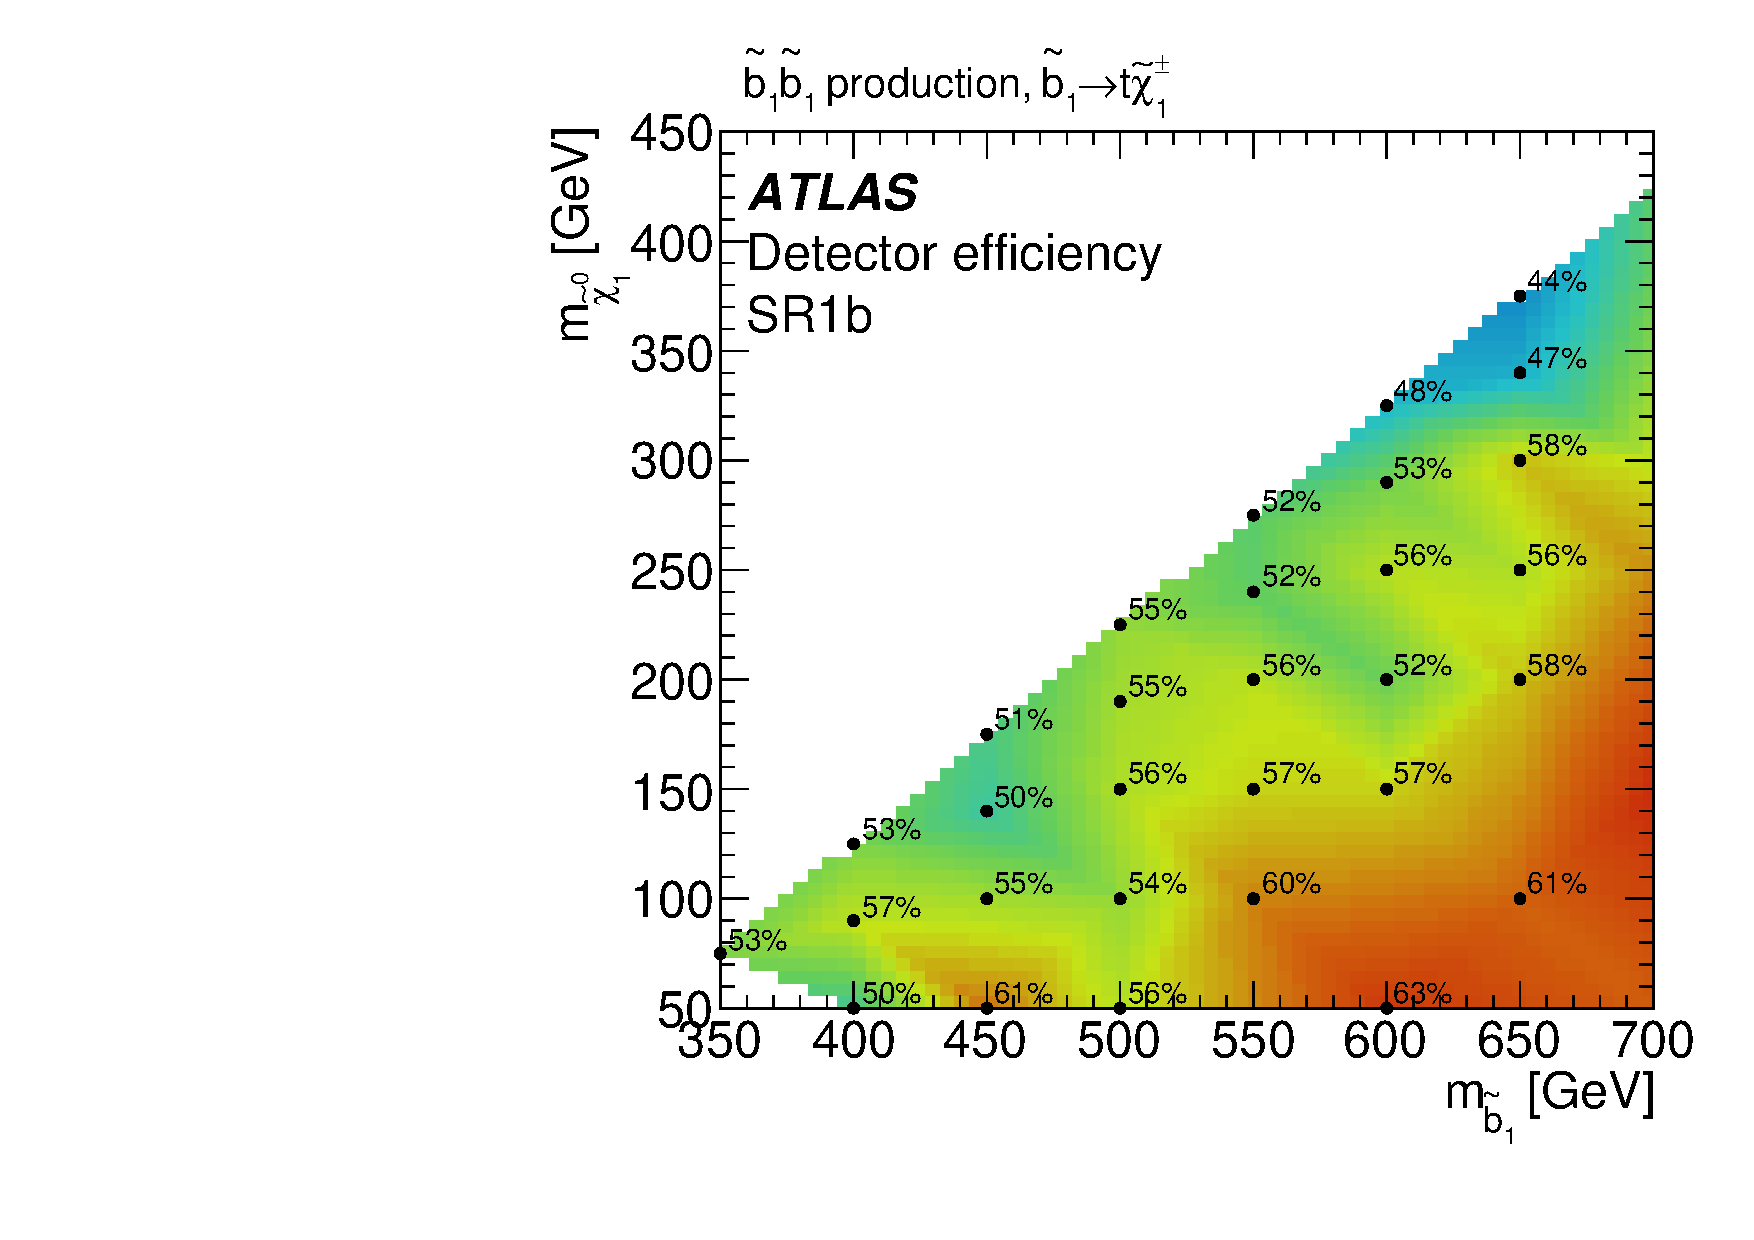
\includegraphics[width=0.37\textwidth]{PUB/FIGURES/HEPDATA/efficiency_SR1b.pdf}}
\subfigure{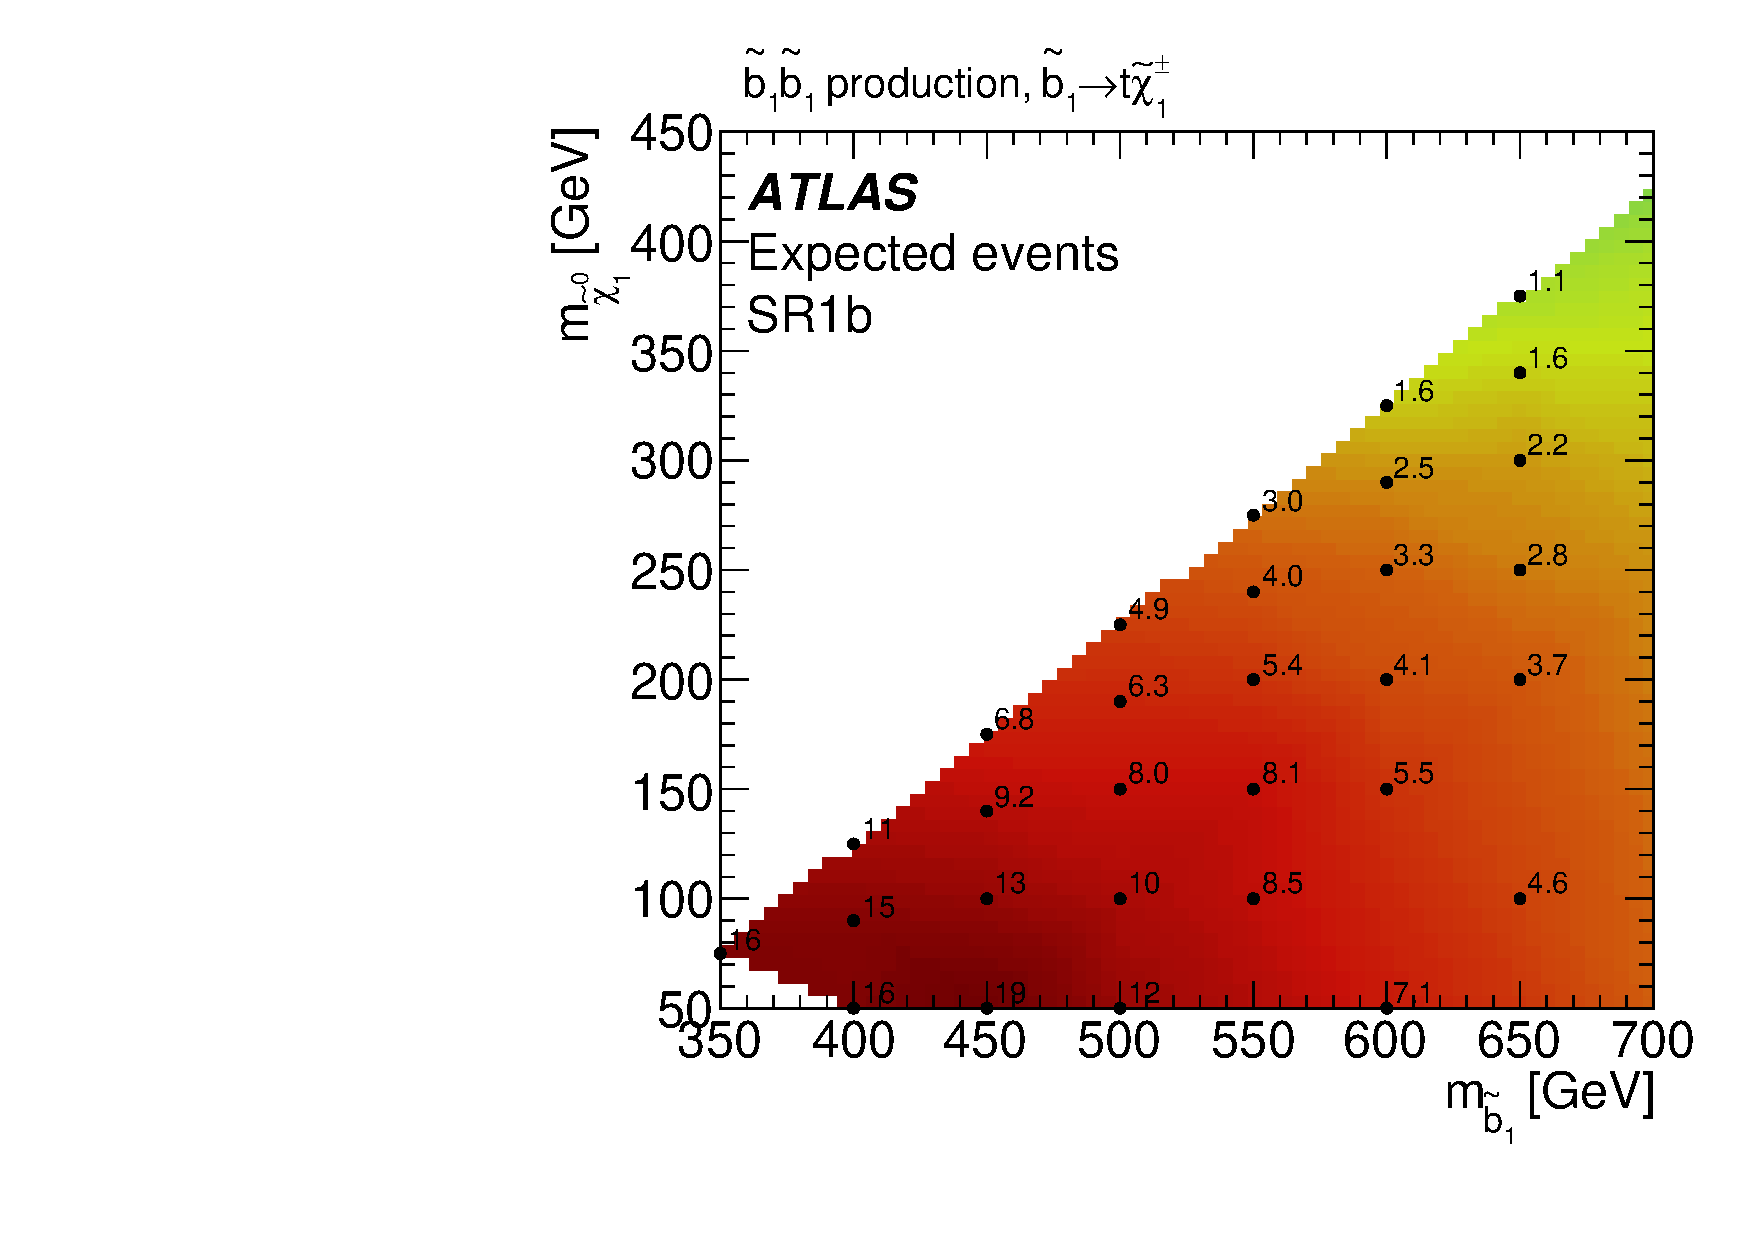
\includegraphics[width=0.37\textwidth]{PUB/FIGURES/HEPDATA/yield_SR1b.pdf}}
\subfigure{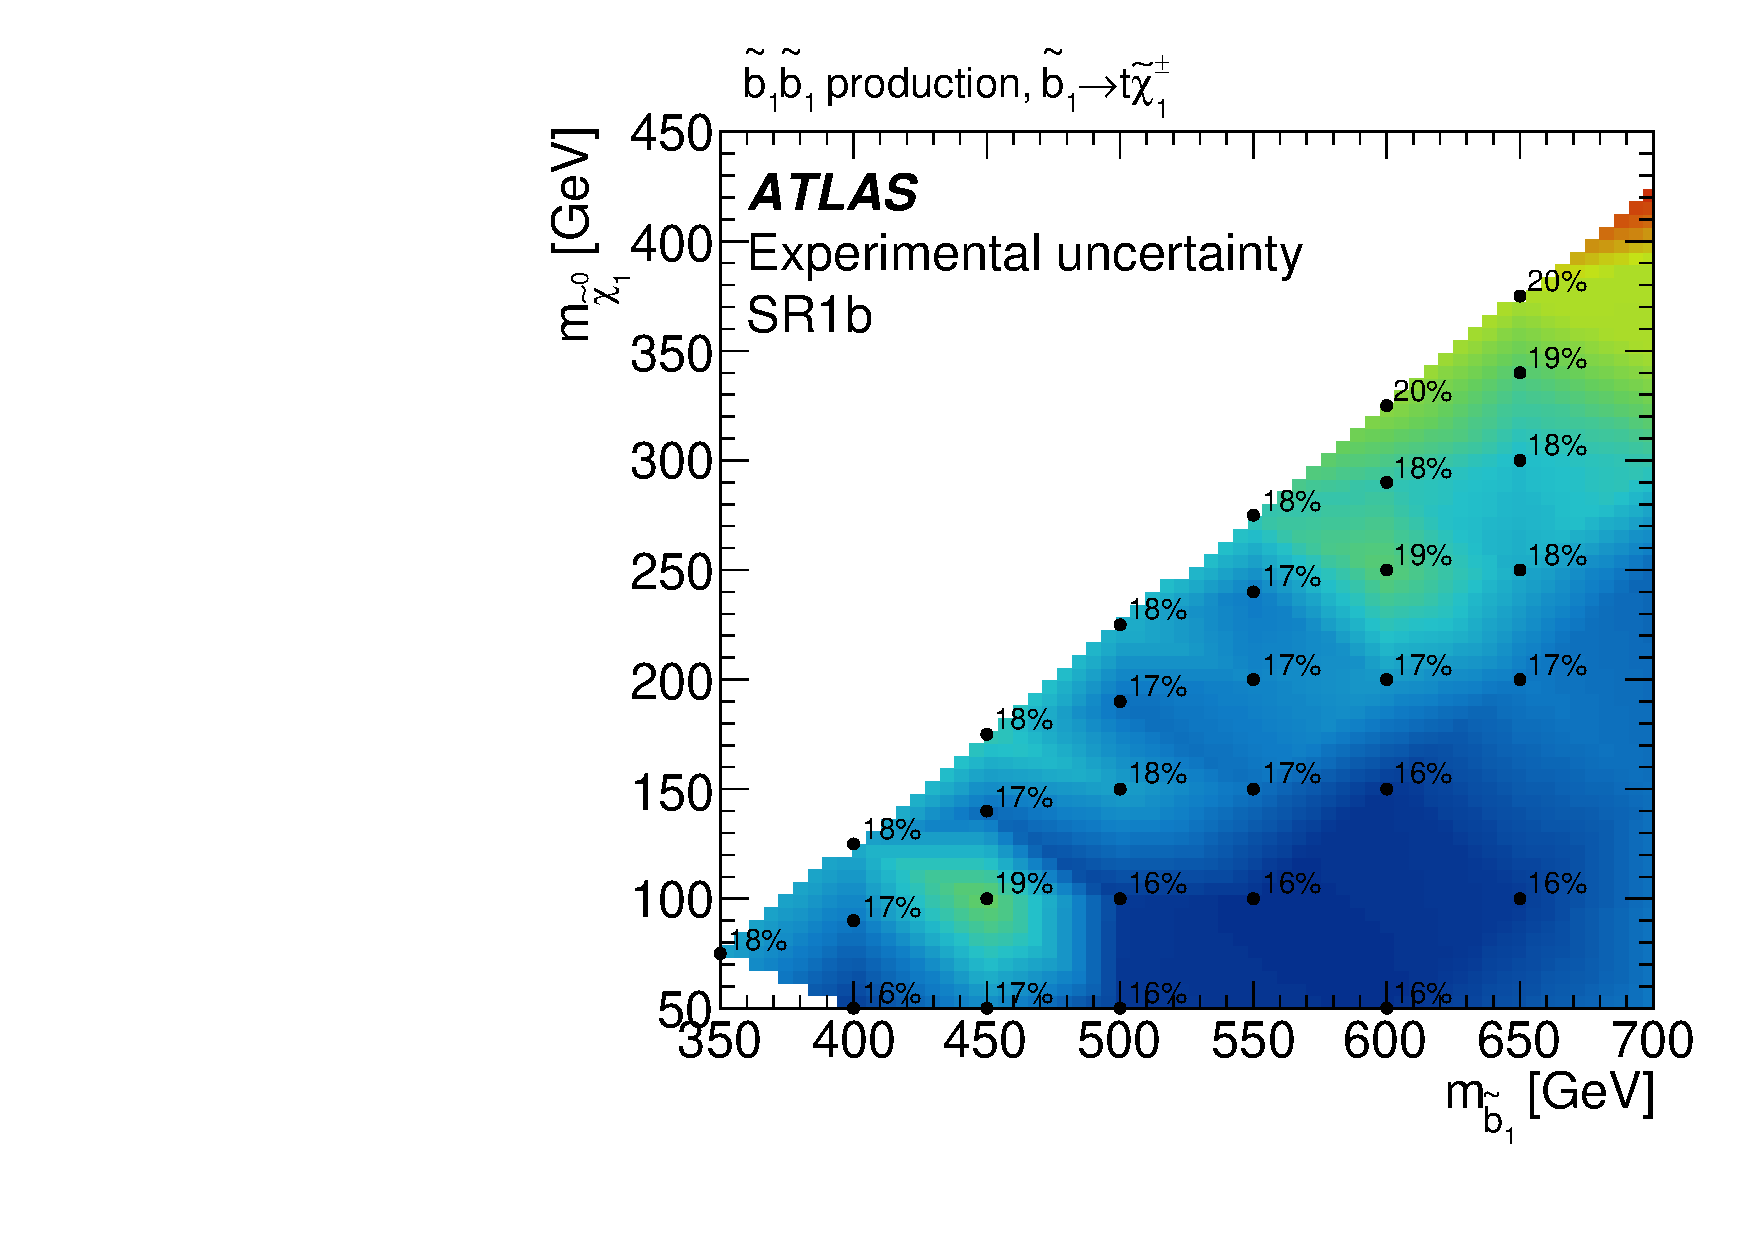
\includegraphics[width=0.37\textwidth]{PUB/FIGURES/HEPDATA/mcsyst_SR1b.pdf}}
\caption{SUSY scenario with $\sbottomone\sbottomone$ production and $\sbottomone\to tW\ninoone$ decay: 
production cross-section (top left), number of generated MC events (top right), 
signal acceptance (middle left) and reconstruction efficiency (middle right) in the signal region SR1b, 
corresponding expected signal yield (bottom left) and associated uncertainty due to experimental sources (bottom right). 
The benchmark scenarios used to set exclusion limits are materialized by black dot markers. 
Acceptance and efficiency are defined as in appendix~A of~\cite{SUSY-2013-19}.}
\label{HEPData_SR1b} 
\end{figure}

% SR3b PUB/FIGURES/HEPData plots
\begin{figure}[p]
\centering
\subfigure{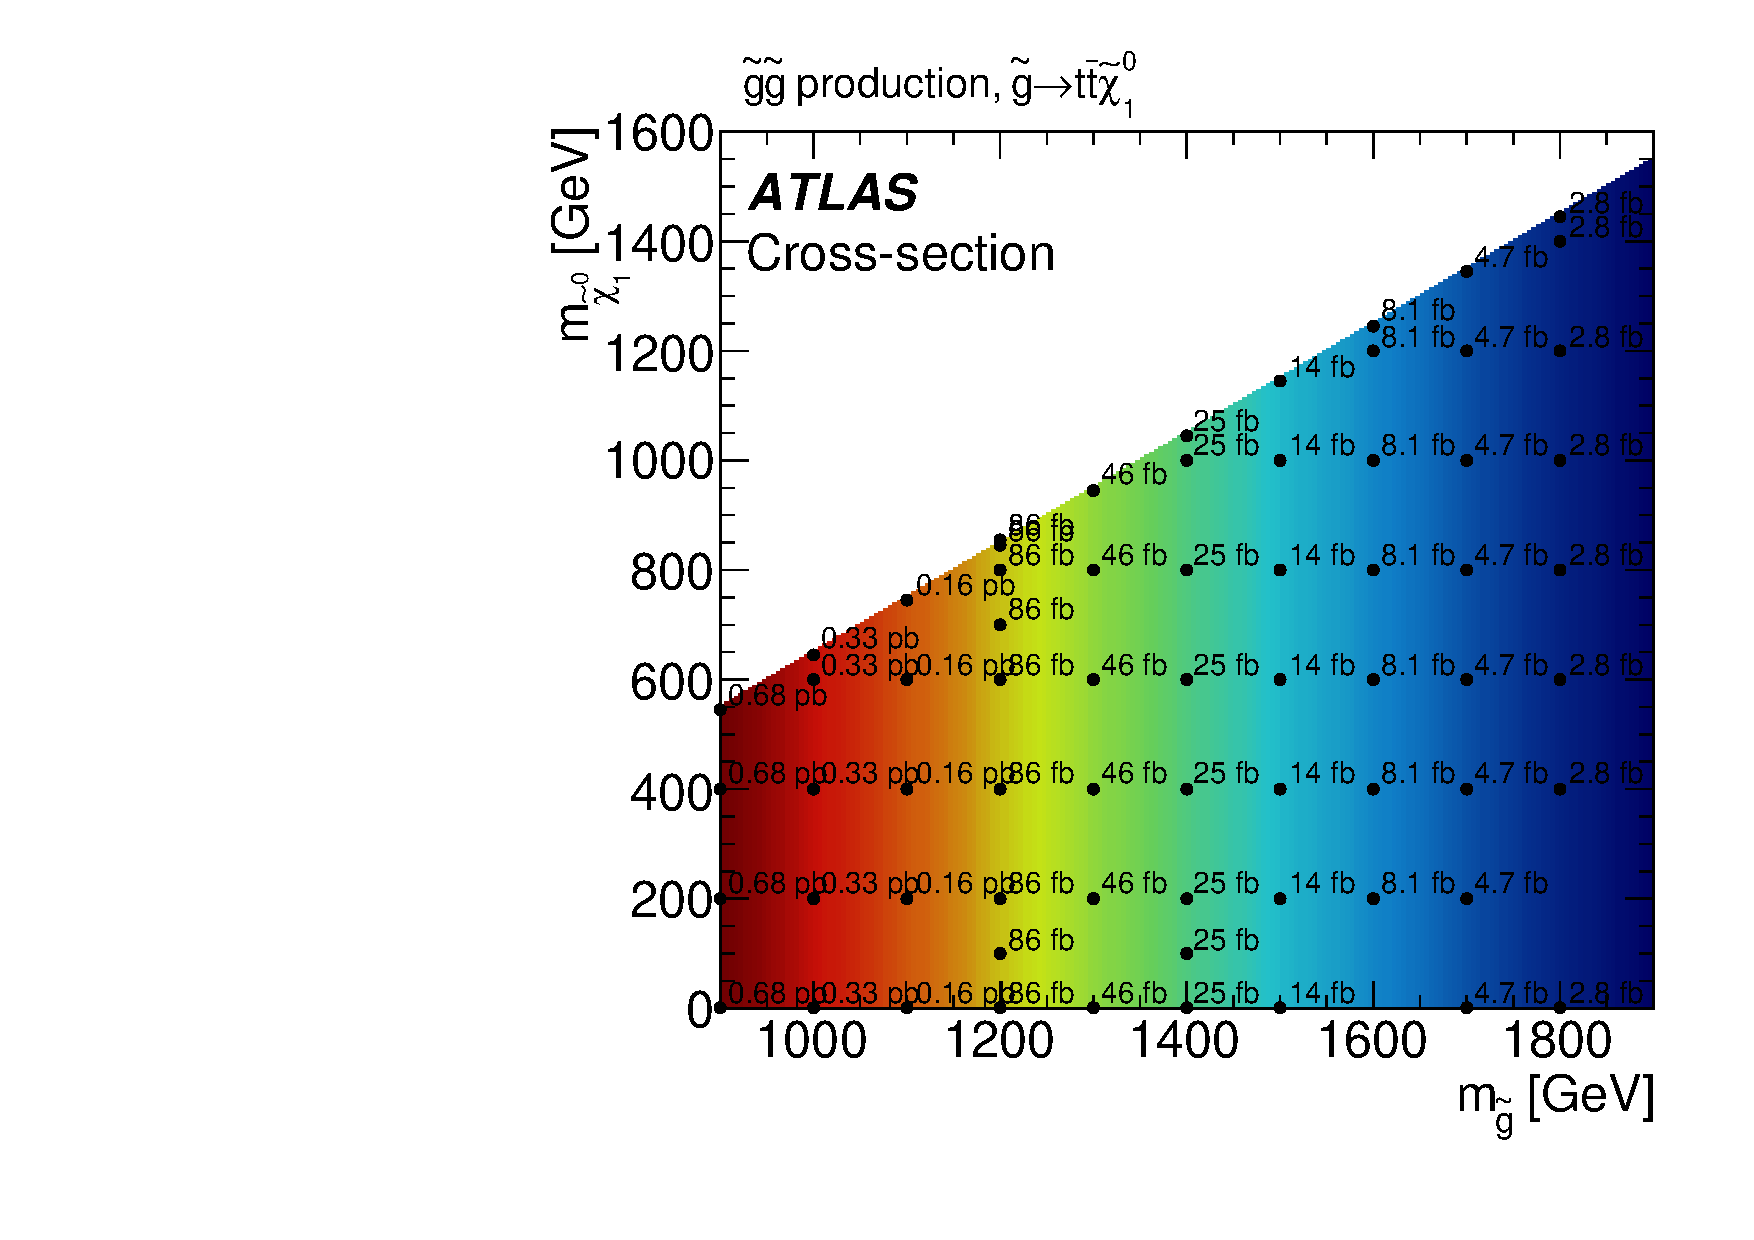
\includegraphics[width=0.37\textwidth]{PUB/FIGURES/HEPDATA/xsection_SR3b.pdf}}
\subfigure{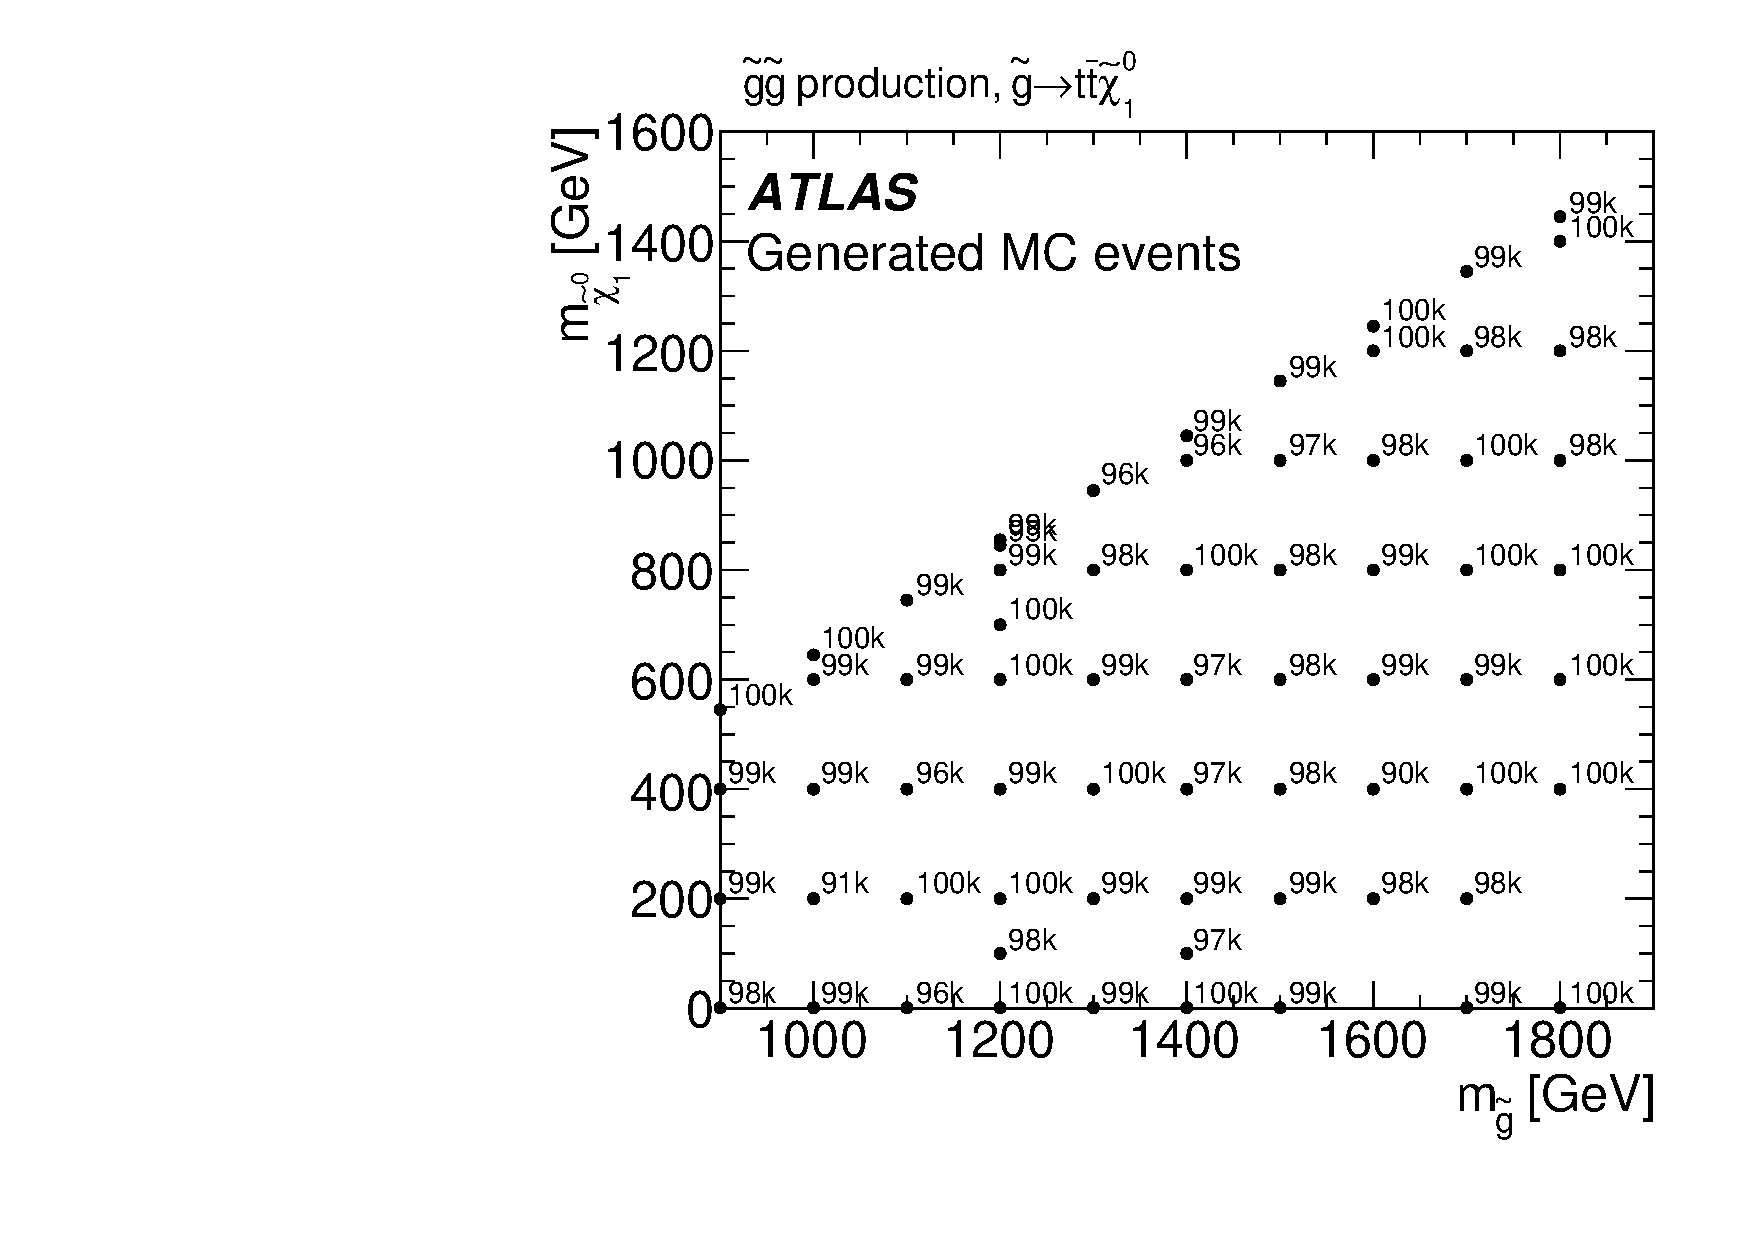
\includegraphics[width=0.37\textwidth]{PUB/FIGURES/HEPDATA/mcstats_SR3b.pdf}}
\subfigure{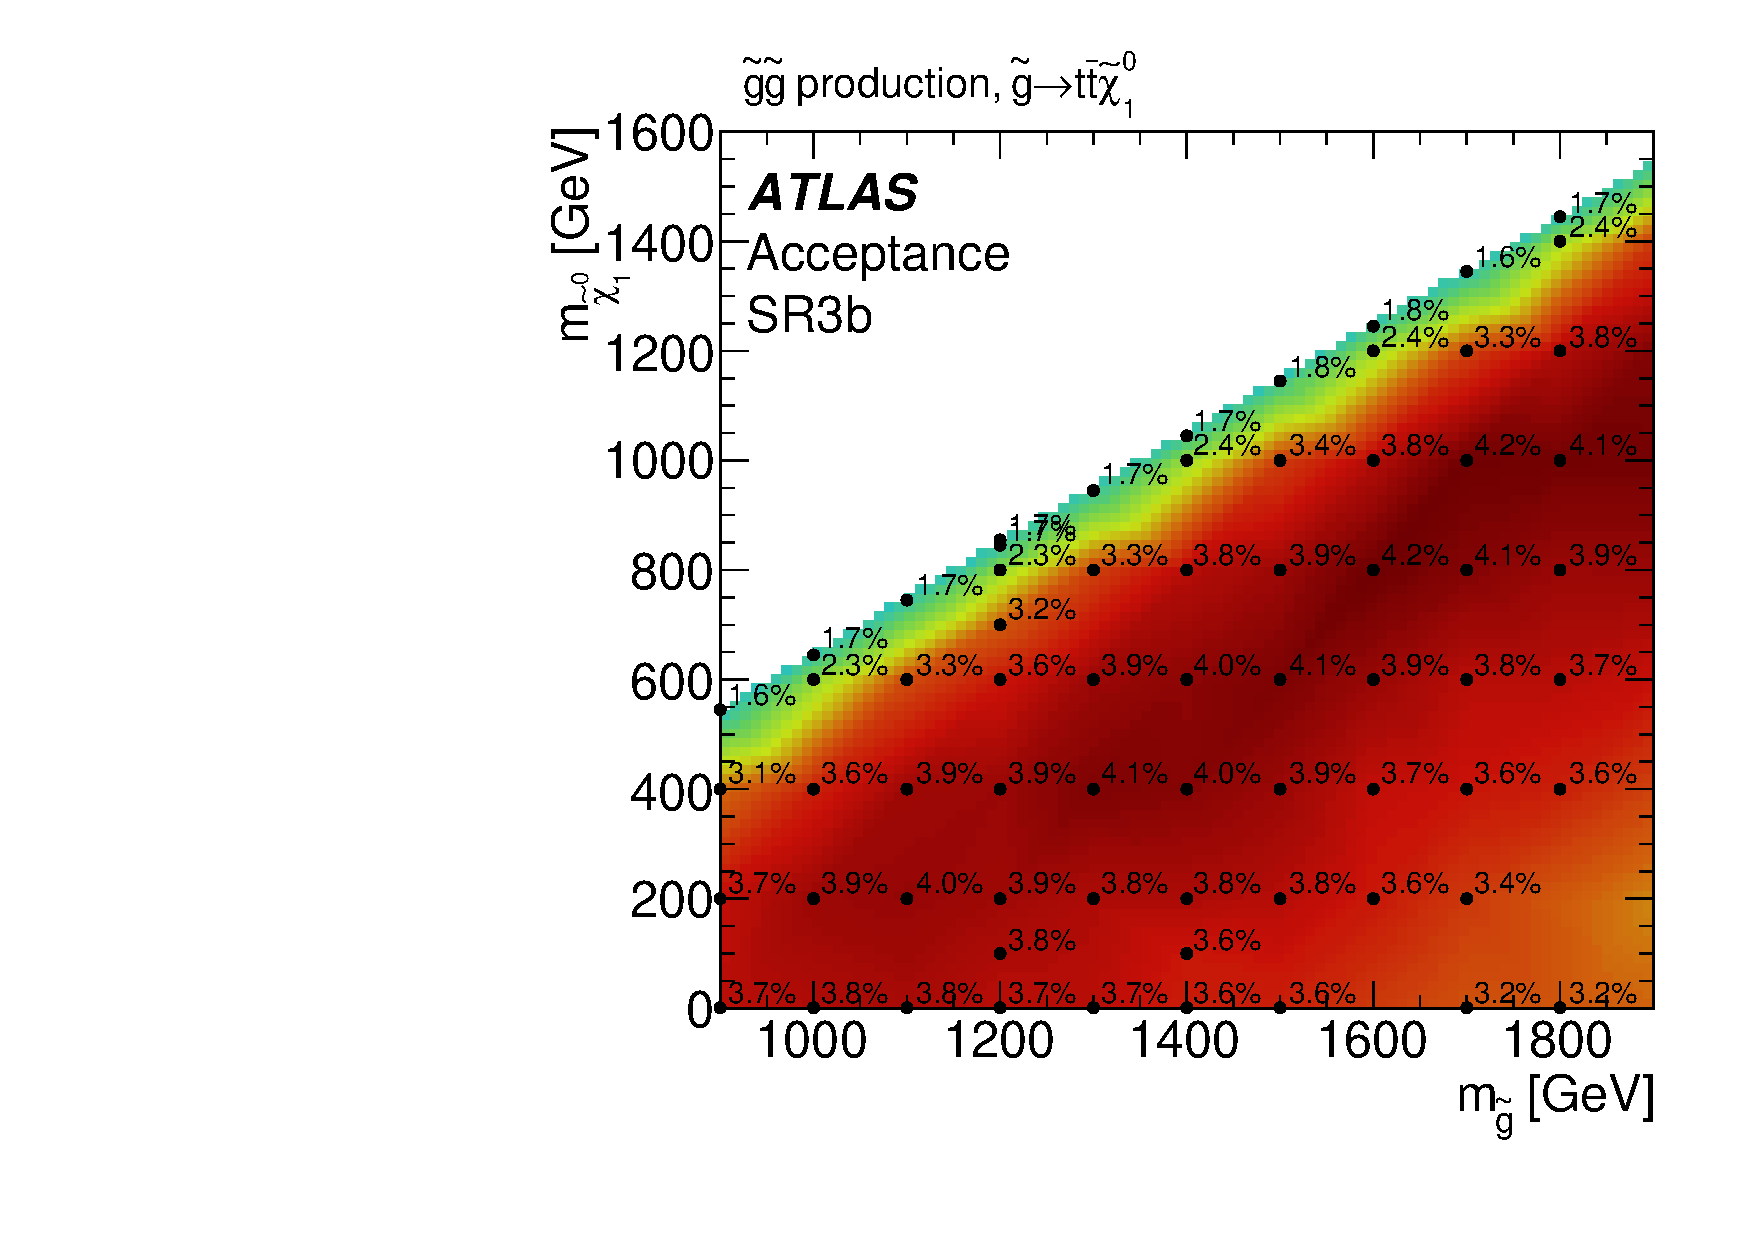
\includegraphics[width=0.37\textwidth]{PUB/FIGURES/HEPDATA/acceptance_SR3b.pdf}}
\subfigure{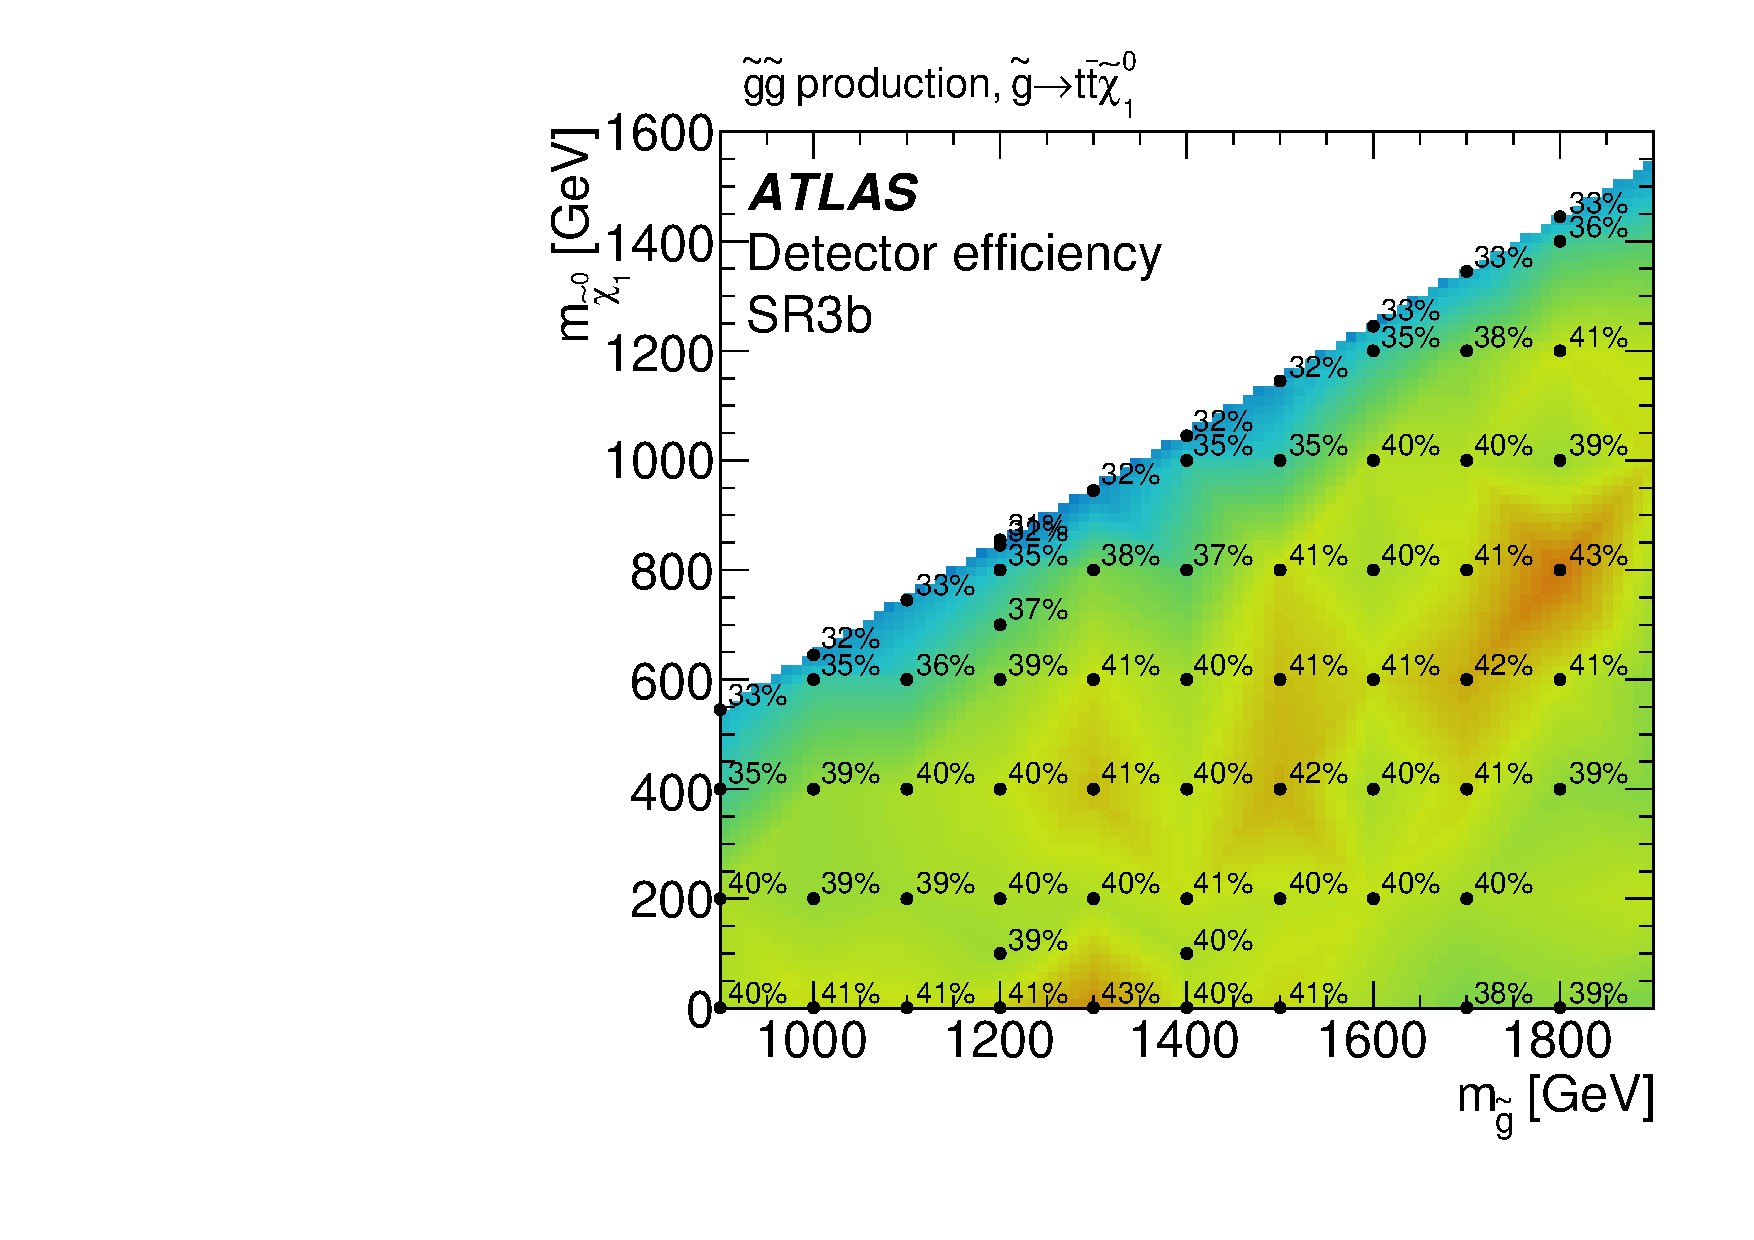
\includegraphics[width=0.37\textwidth]{PUB/FIGURES/HEPDATA/efficiency_SR3b.pdf}}
\subfigure{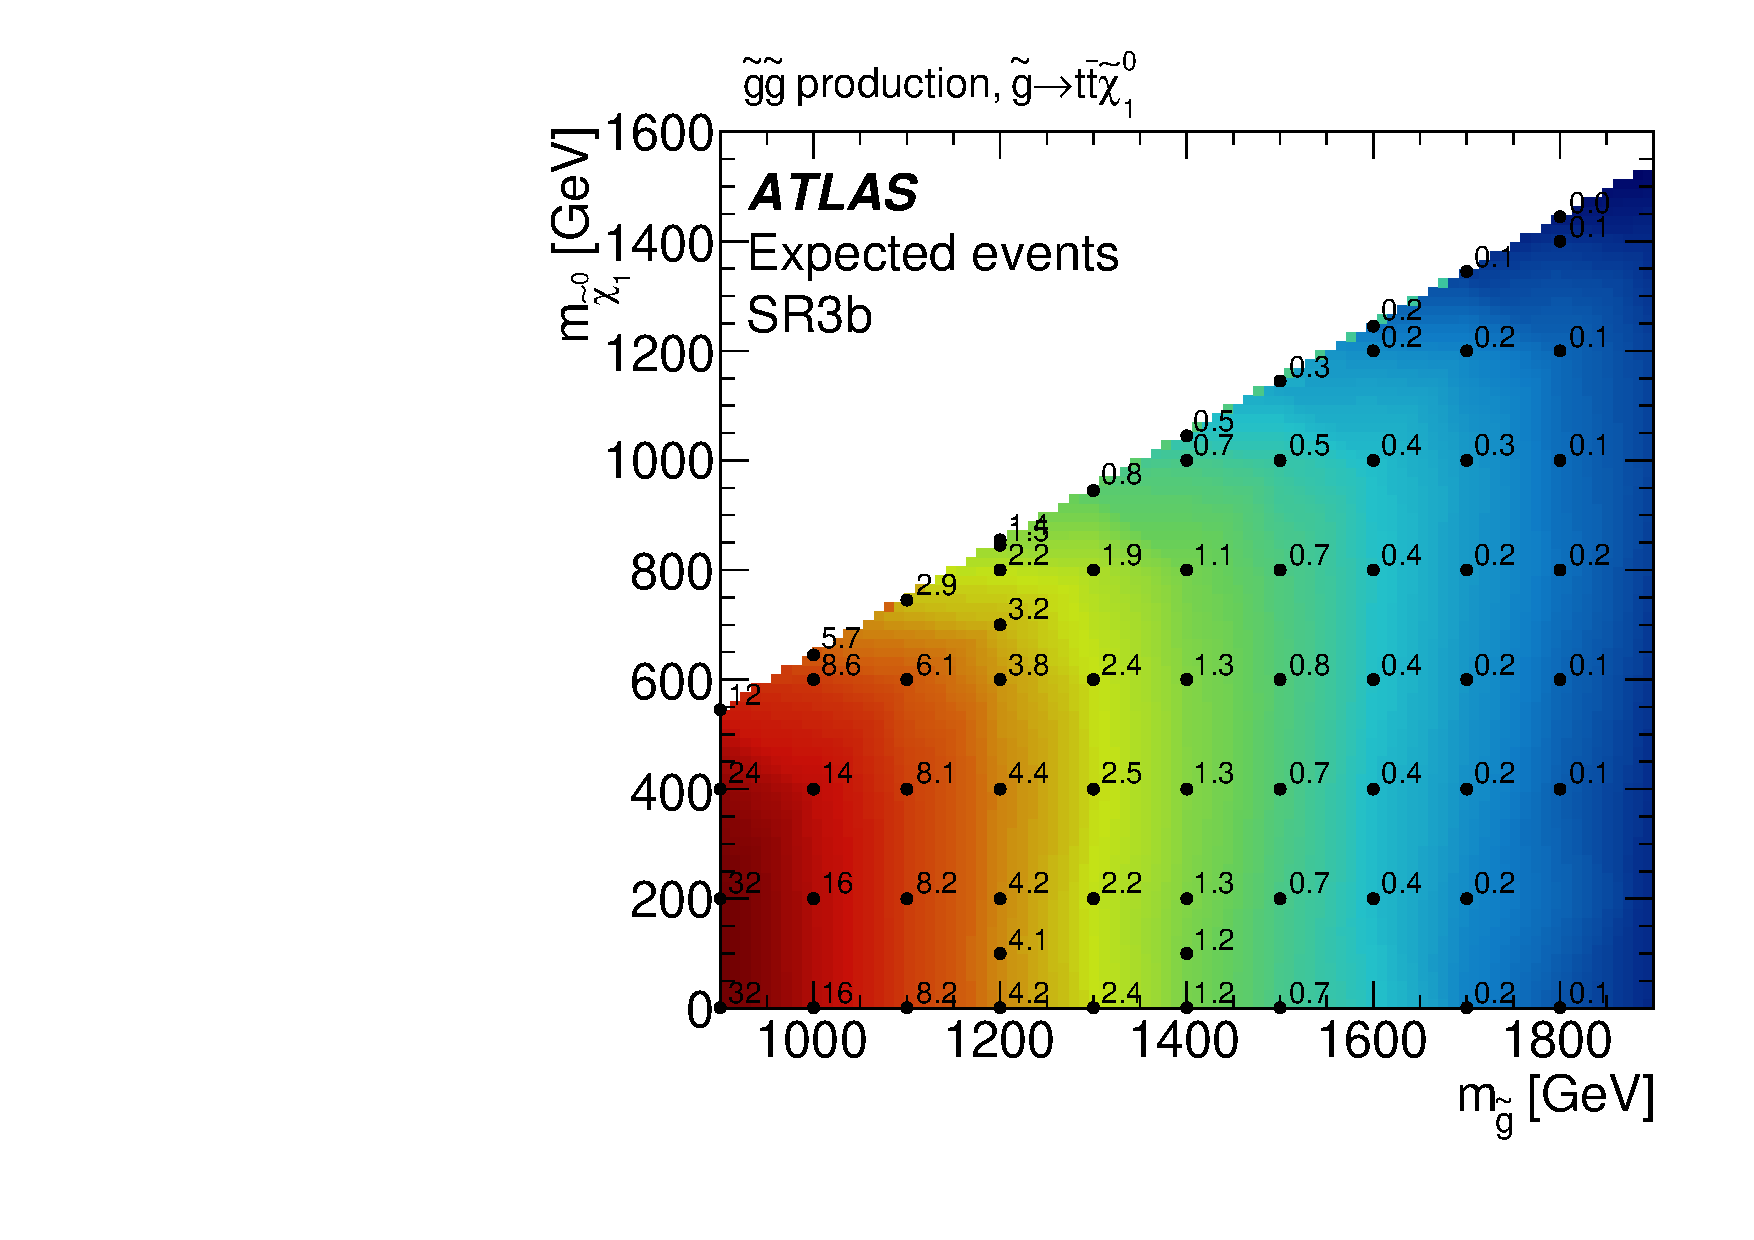
\includegraphics[width=0.37\textwidth]{PUB/FIGURES/HEPDATA/yield_SR3b.pdf}}
\subfigure{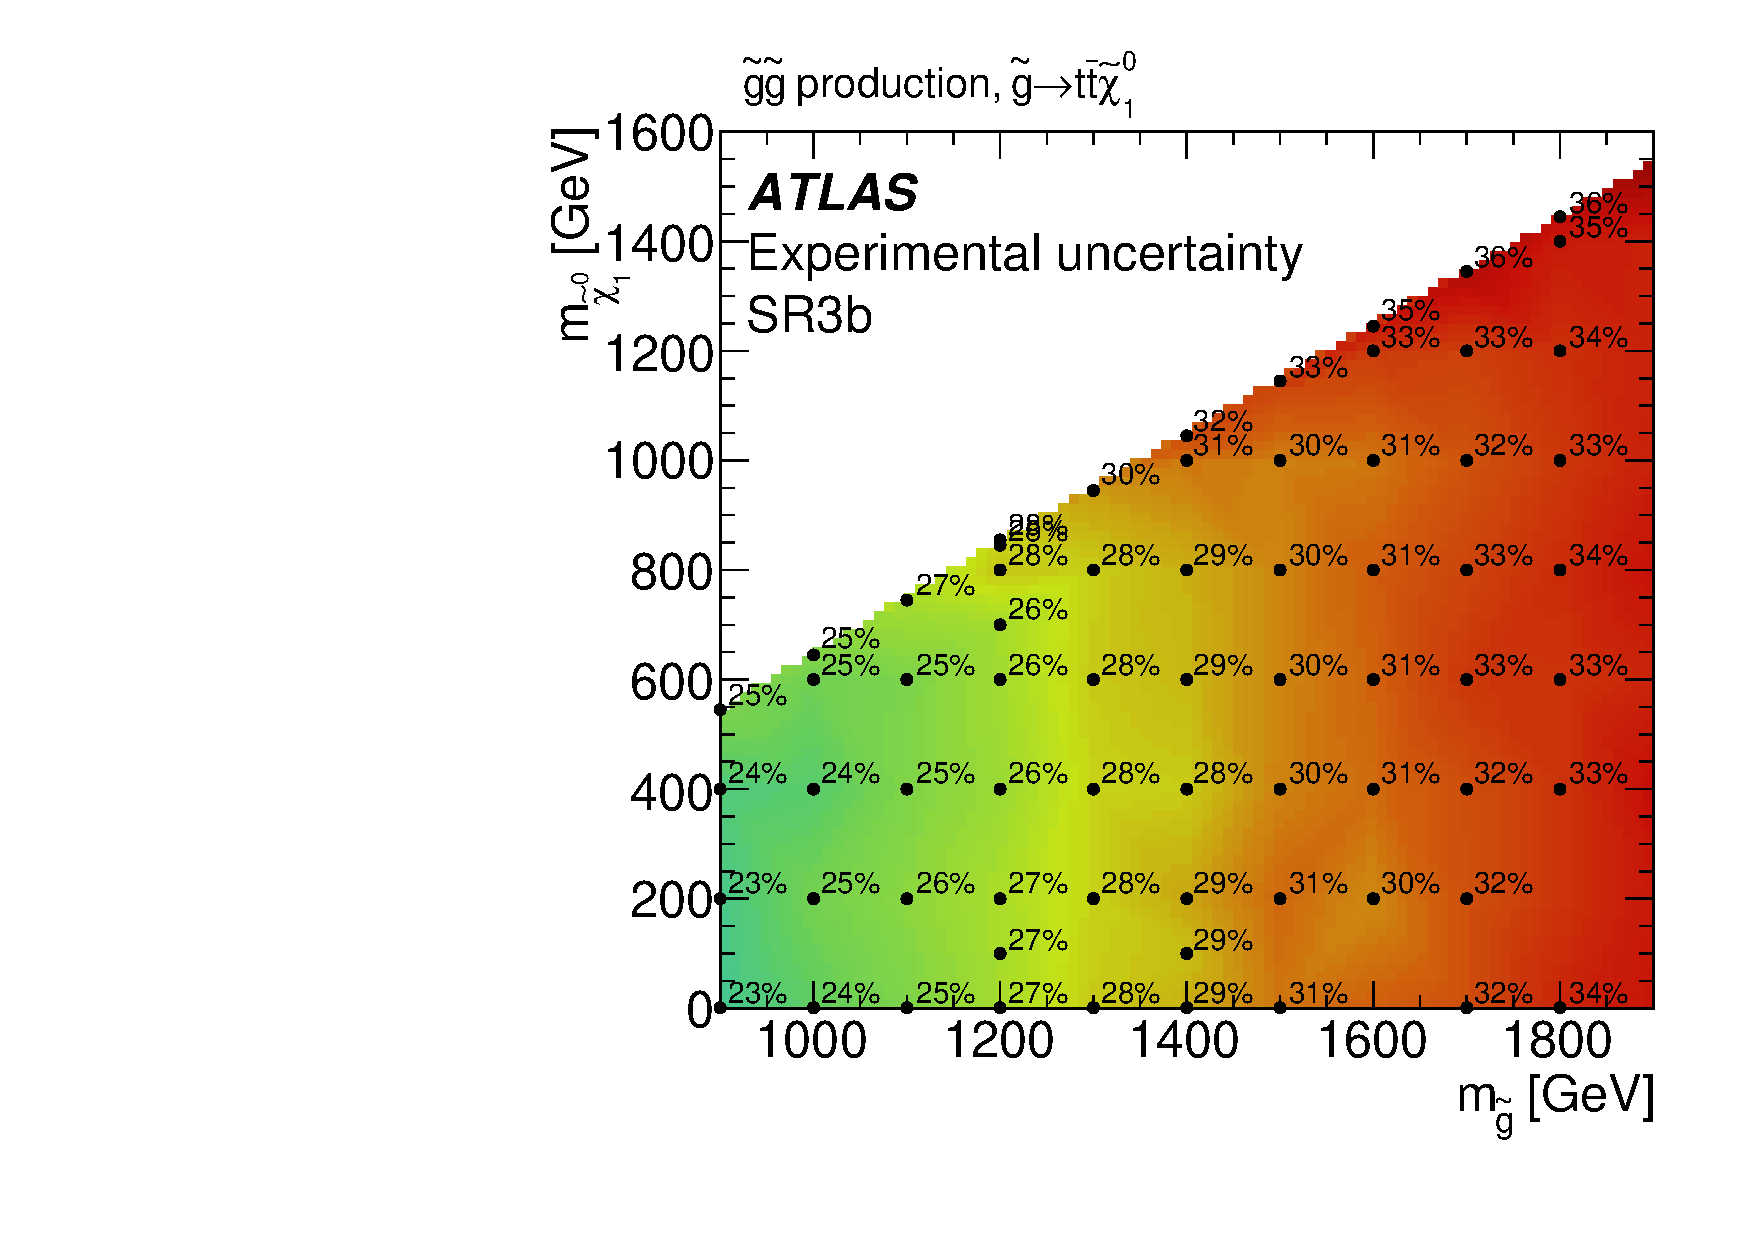
\includegraphics[width=0.37\textwidth]{PUB/FIGURES/HEPDATA/mcsyst_SR3b.pdf}}
\caption{SUSY scenario with $\gluino\gluino$ production and $\gluino\to t\bar t\ninoone$ decay: 
production cross-section (top left), number of generated MC events (top right), 
signal acceptance (middle left) and reconstruction efficiency (middle right) in the signal region SR3b, 
corresponding expected signal yield (bottom left) and associated uncertainty due to experimental sources (bottom right). 
The benchmark scenarios used to set exclusion limits are materialized by black dot markers. 
Acceptance and efficiency are defined as in appendix~A of~\cite{SUSY-2013-19}.}
\label{HEPData_SR3b} 
\end{figure} 
